\documentclass{report}
\usepackage{suthesis-2e}
%\documentclass[a4paper]{article}
\usepackage{positivesubtyping}

\title{Type Inference in Presence of Positive Subtyping\\with Bounded Quantification}
\author{Kathleen Fisher and Pascal-Louis Perez}
\date{June 7, 2007}

% document
\begin{document}
  \maketitle
  
  \begin{abstract}
     We investigate the introduction of a positive subtyping relation
     in a Hindley/Milner style type inference. Positive subtyping is a restricted
     form of the standard contra-variant subtyping and makes type inference
     algorithmically more efficient. By itself, positive
     subtyping is not as expressive as one would hope and
     we present a constraint-based syntax-directed type inference system targeted at
     improving this expressiveness. We extend this type inference system with
     declarative rules simplifying its presentation and give a formal comparison
     between our system and Hindley/Milner style type systems.
     In particular, we prove that subtyping can be incorporated into an existing type system
     whilst preserving the complexity class of type inference. We show that in our
     setting, satisfiability of inequalities is PTIME-complete. Finally, we use a constraint
     satisfaction algorithm and show its application to our type system.
  \end{abstract}
  
  \prefacesection{Acknowledgments}
    All my gratitude goes to Kathleen Fisher for making this research possible.
    In the early steps of this research, she gave me a lot of liberty to explore
    potential directions and provided me with crucial insights. She was flexible
    enough to allow me to work remotely despite the extra workload this
    represented for her. During the elaboration of the type inference system,
    her intuition and knowledge got me out of difficult proofs and bad directions.
    \\
    \par\noindent\noindent\ignorespaces Thanks goes to Alex Aiken and 
    John C. Mitchell, my two advisors, for
    enabling me to pursue the Distinction in Research during my Masters.
    I also thank Professor Mitchell for his financial support.
    \\
    \par\noindent\noindent\ignorespaces I am thankful to Martin Odersky
    and Uwe Nestmann for introducing me to programming language theory and
    sharing with me their passion. I also thank, in no specific order,    
    Marcin Benke, Fran\c{c}ois Pottier, Didier R\'emy, John Reppy and Martin Sulzmann
    for their various contributions.
    \\
    \par\noindent\noindent\ignorespaces Last, I would also like to thank
    Thibault Guicherd-Callin for proof-reading
    this thesis alongside of his time consuming projects.
    \\
    \par\noindent\noindent\ignorespaces Finally, I would like to thank
    my wife Dalia and daughter Aline for their
    patience, as well as the rest of my family for making my studies at Stanford
    University possible.
  \tableofcontents
  
  \chapter{Introduction}
  Since its discovery, Hindley/Milner style type inference systems have been a popular approach to
  handling types in functional programming languages and has evolved rapidly. These type systems
  share totality and thus allow the programmer to omit all type annotations. This approach
  is challenging and many extensions have been shown intractable or undecidable (such as
  arbitrary-rank types \cite{kfoury:rank2}).
  
  In this work, we consider the problem of type inference in the presence of positive
  subtyping. Subtyping captures the type safety of substitutability of an expression and arises
  naturally in object-oriented languages.
  In essence, an expression $e_1$ can be safely substituted for $e_2$, if $e_1$'s type
  is a subtype of $e_2$'s type. From an information theoretic view, subtyping can be seen as a
  ``more informative'' or ``more precise'' relation.
  
  Functional subtyping considers the relation between two functional types and exhibits
  algebraic difficulties. Take a function $f$ of type $\type{A}\fun\type{B}$ used in some context $E$ forming the
  expression $E[f]$. The function $f$ may be applied to any expression with type $\type{A}$
  and produces an expression of type $\type{B}$. Therefore, we can substitute for $f$ a function that produces
  subtypes of $\type{B}$ since these will be safely used in the context. Similarly,
  we can substitute for $f$ a function expecting supertypes of $\type{A}$ as within the context $E$,
  the function is applied to expressions with type $\type{A}$. Indeed, expressions with type $\type{A}$
  are safe substitutes
  in a context that expects a supertype of $\type{A}$.
  
  We can observe that the functional subtyping relation is co-variant, or positive,
  in the return type and contra-variant,
  or negative, in the argument type. Hoang and Mitchell \cite{hoang:thesis,hoang:lower-bounds}
  have shown that constraint satisfaction
  in presence of the standard contra-variant subtyping relation can be PSPACE-hard. We study the restriction
  of the subtyping relation by disallowing contra-variance, and call this positive subtyping.
  In a positive subtyping relation, types vary only co-variantly or positively.
  For functional subtyping, the argument type becomes invariant and the return type stays co-variant.
  The positive subtyping relation is a strict subset of the standard subtyping relation.
  
  We discuss the challenges introduced by the loss of expressiveness
  and use constrained type schemes $\forall\bar{\type{X}}|C.\type{T}$ to recover a restricted
  form of contra-variance. Constraints are built from subtyping constraints and conjunctions.
  We add for presentation and for semantic arguments the predicate $\true$ and $\false$
  with the usual meaning as well as existential quantification. We interpret constraints
  by grounding them, making their interpretation a natural extension of the subtyping relation
  and logical conjunction. Type schemes' interpretation follows from the meaning of constraints.
  
  We present a syntax-directed type inference system in the line of HM(X)
  \cite{sulzmann97type}. An alternative declarative version is given. This alternative
  presentation simplifies the understanding of the
  algorithmic presentation whilst preserving structural properties.
  In addition, the declarative formulation allows a programmer to reason about the type system
  as if it were a standard object-oriented type system, in which constraints are present
  to recover expressiveness, not for typing subtleties.
  We give a formal comparison between our system and Hindley/Milner style type systems
  and show that our type system is a strict extension.
  
  We then show that positive subtyping can be incorporated into an existing type
  system whilst preserving the complexity class of type inference. In fact, positive
  subtyping lifts the subtyping relation without altering the shape of the
  ordering relation. In our setting, satisfiability of inequalities
  is PTIME-complete.
  
  Finally, we adapt a constraint satisfaction algorithm, developed
  by Benke \cite{benke93} to verify the satisfiability of constraints gathered
  during type inference and thus verify that programs are well-typed.
  A prototype implementation of our system
  is available on \url{http://www.stanford.edu/~plperez/} and we give a few examples
  in appendix.
  
  \section{Expressiveness}
  Positive subtyping is a strict subset of the usual notion of subtyping and
  is therefore over-protective. It prevents safe substitutions and is especially
  noticeable with higher-order
  functions. For instance, one might need to use points as keys in a hash table and
  thus hash point objects. From an implementation point of view, one needs a
  $\type{Point}\fun\Int$ hash function, but from a client's perspective a
  generic hash function $\type{Object}\fun\Int$ may be sufficient.
  Because of positive subtyping, simple mismatch, such as the one we highlighted,
  prevents the typability of the program. Hofmann and Pierce
  \cite{pierce:positive-subtyping} nonetheless note that this weaker relation
  retains sufficient flexibility to model objects, encapsulation and inheritance.
  
  Formalizing the preceding example, consider a version of the
  apply function $\lambda x.\lambda f.f\ x$, taking a value followed by
  a function and applying the function to the value. With a standard contra-variant subtyping
  relation, the type $\forall\type{X},\type{Y}.\type{X}\fun(\type{X}\fun\type{Y})\fun\type{Y}$ is
  expressive enough. If the value is a colored point $c$, we have $\lambda f.f\ c$
  whose type is now
  \begin{displaymath}
    \forall\type{Y}.(\type{ColoredPoint}\fun\type{Y})\fun\type{Y}
  \end{displaymath}
  since $\type{X}$ has been instantiated to $\type{ColoredPoint}$. With positive subtyping,
  only functions whose domain is \type{ColoredPoint} are admissible.
  
  The decoupling between the type derivation of apply to $c$ and the resulting expression
  to a function $f$ introduces additional difficulty. If the two applications
  were typed together in one derivation, one could instantiate $\type{X}$ to $f$'s argument type.
  
  We can see in apply's type
  \begin{displaymath}
    \forall\type{X},\type{Y}.\underline{\type{X}}\fun(\underline{\type{X}}\fun\type{Y})\fun\type{Y}
  \end{displaymath}
  that the two $\type{X}$'s are unnecessarily coupled together. A looser approach would
  number them $\type{X}_1$ and $\type{X}_2$ and require that $\type{X}_1\subtype\type{X}_2$.
  Introducing bounded quantifiers allows having a positive subtyping relationship 
  and yet use a restricted form of contra-variance. Continuing the previous example, we have
  \begin{displaymath}
    \forall\bar{\type{X}},\type{Y}|\type{X}_1\subtype\type{X}_2.\type{X}_1\fun(\type{X}_2\fun\type{Y})\fun\type{Y}
  \end{displaymath}
  which allows us to add extra liberty to cope with the loss of positive subtyping.
  If we now consider a higher-order case, with a length function $l$ of type $\type{Point}\fun\Int$,
  we have
  \begin{displaymath}
    \lrp{\lambda x.\lambda f.f\ x}\ l : \forall\type{Y}.\lrp{\lrp{\type{Point}\fun\Int}\fun\type{Y}}\fun\type{Y}
  \end{displaymath}
  since the constraint $\type{Point}\fun\Int\subtype\type{X}_2$ forces $\type{X}_2$ to be
  equated with $\type{Point}\fun\Int$. Here, positive subtyping leads to a restrictive type. One could transform this
  partially grounded type based on a variance analysis to
  \begin{displaymath}
    \forall\type{X},\type{Y}|\type{X}\subtype\type{Point}.\lrp{\lrp{\type{X}\fun\Int}\fun\type{Y}}\fun\type{Y}
  \end{displaymath}
  but we do not consider this extension in this work. Another challenge
  with an object-oriented type system is heterogeneous collections.
  Suppose we have a sequencing operator $e_1;e_2$ which is syntactic sugar
  for $\lambda x.e_2\ e_1$ for an $x$ not appearing in $e_2$. We can define
  an apply twice function $\lambda x_1.\lambda x_2.\lambda f.f\ x_1;f\ x_2$
  taking two values $x_1$, $x_2$ and a function $f$ applied sequentially
  to the two values. The Hindley/Milner type is
  \begin{displaymath}
	  \forall\type{X},\type{Y}.\type{X}\fun\type{X}\fun(\type{X}\fun\type{Y})\fun\type{Y}
  \end{displaymath}
  whose rigidity is very limiting. Instead, using bounded quantifier one
  might have
  \begin{displaymath}
	  \forall\bar{\type{X}},\type{Y}|\type{X}_1\subtype\type{X}_3\land\type{X}_2\subtype\type{X}_3.\type{X}_1\fun\type{X}_2\fun(\type{X}_3\fun\type{Y})\fun\type{Y}
  \end{displaymath}
  allowing independent type derivations without preventing further uses.
  
  \section{Row Polymorphism}
  Another approach adds positive subtyping to row polymorphism. Rows were introduced
  by R\'emy \cite{projectiveml} and are described thoroughly in Pottier and R\'emy \cite{pottier-remy-emlti}.
  A row $\Pi R$ is an infinite support record.
  We denote a single labeled type by $l:\type{T}$ and the infinite part
  of $\Pi R$ by $\delta\type{T}$. A typical one-dimensional point object whose
  record type is $\set{x:\Int}$ would have a row type $\Pi(x:\Int,\delta\top)$,
  and a selection function $\lambda x.x.l$ would have a polymorphic row type
  $\forall\bar{\type{X}}.\Pi(l:\type{X}_1,\type{X}_2)\fun\type{X}_1$ where the kind
  of $\type{X}_2$ is a partial row on $\Labels\setminus\set{l}$.
  
  By analogy with records, we can extend the subtyping relation to rows
  by considering a row $\Pi R_1$ a subtype of $\Pi R_2$
  if all types in $R_1$ are subtypes of $R_2$ with a label-wise comparison;
  for example $\Pi(x:\Int,y:\Bool,\delta\top)$ is a subtype of $\Pi(x:\Int,\delta\top)$.
  
  This approach is more expressive than plain positive subtyping. Nonetheless, similar difficulties
  as the one discussed previously arise, especially with heterogeneous collections.
  
  \chapter{Syntax}
  We consider a slightly extended version of the simply typed $\lambda$-calculus with constants,
  record construction and record selection. Records are introduced as a means for structural subtyping.
    
  \section{Expressions}
  The expressions we consider are generated by the grammar
  \begin{displaymath}
    e \eqg c
      \mid x
      \mid \lambda x.e
      \mid \eapp{e_1}{e_2}
      \mid \elet{x}{e_1}{e_2}
      \mid \set{\vec{l}=\vec{e_l}}
      \mid \esel{e}{l}\textrm{.}
  \end{displaymath}
  We have constants (denoted by $c$\notation{ec}), variables (denoted by
  $x$\notation{ex}), anonymous functions ($\lambda x.e$), application ($\eapp{e_1}{e_2}$),
  let polymorphism ($\elet{x}{e_1}{e_2}$), record expressions ($\set{\vec{l}=\vec{e_l}}$)
  and finally record selection ($\esel{e}{l}$). Record labels $l$\notation{label}
  are chosen from a set of labels $\Labels$\notation{labels}, which is infinite but denumerable.
  \begin{dfn}
    The free variables $\fv$\notation{fv} of an expression $e$ is defined inductively by
    \begin{mathpar}
      \fv(c)=\emptyset \and
      \fv(x)=\set{x} \and
      \fv\lrp{\lambda x.e}=\fv(e)\setminus\set{x} \and
      \fv\lrp{\eapp{e_1}{e_2}}=\fv(e_1)\cup\fv(e_2) \and
      \fv\lrp{\elet{x}{e_1}{e_2}}=\fv(e_1)\cup\fv(e_2)\setminus\set{x} \and
      \fv\lrp{\set{\vec{l}=\vec{e_l}}}=\bigcup_{l\in\bar{l}}\fv(e_l) \and
      \fv\lrp{\esel{e}{l}}=\fv(e)
    \end{mathpar}
  \end{dfn}
  
  \section{Monomorphic Types}
  The monomorphic types we consider are
  \begin{displaymath}
    \type{T} \eqg \top
             \mid \type{B}
             \mid \type{X}
             \mid \type{T}_1\fun\type{T}_2
             \mid \set{\vec{l} : \vec{\type{T}_l}}\textrm{.}
  \end{displaymath}
  $\type{B}$\notation{tb} ranges over a set of base types (such as $\Int$, $\Bool$
  or $\Char$). We also have type variables represented by $\type{X}$\notation{tv}, functional
  types $\type{T}_1\fun\type{T}_2$ and record types $\set{\vec{l} : \vec{\type{T}_l}}$.
  Finally, the top type $\top$\notation{tt} is a supertype of all types.
  We use $\type{T}$ or $\type{U}$\notation{mono} to range over monomorphic types.
  We refer to the infinite set of type variables as $\TVars$\notation{tvars}
  and refer to the infinite set of monomorphic types generated by the previous
  grammar as $\Types$\notation{types}.
  \begin{dfn}
    The free type variables $\ftv$\notation{ftv} of a monomorphic type $\type{T}$
    is defined inductively by
    \begin{mathpar}
      \ftv(\top)=\emptyset \and
      \ftv(\type{B})=\emptyset \and
      \ftv(\type{X})=\set{\type{X}} \and
      \ftv\lrp{\type{T}_1\fun\type{T}_2}=\ftv(\type{T}_1)\cup\ftv(\type{T}_2) \and
      \ftv\lrp{\set{\vec{l} : \vec{\type{T}_l}}}=\bigcup_{l\in\bar{l}}\ftv(\type{T}_l)
    \end{mathpar}
  \end{dfn}
  \begin{dfn}
    We define the set of ground types $\GTypes$\notation{gtypes} as
    \begin{displaymath}
      \GTypes = \coll{\type{T}\in\Types}{\ftv(\type{T})=\emptyset}
    \end{displaymath}
    that is all types not containing any type variable. A ground type is a type
    contained in $\GTypes$.
  \end{dfn}
  
  \section{Polymorphic Types}
  \begin{eqnarray}
    \type{S} &\eqg& \forall\bar{\type{X}}|C.\type{T}\textrm{.}\nonumber\\
    C        &\eqg& \true
               \mid \false
               \mid \type{T}_1\subtype\type{T}_2
               \mid C_1 \land C_2
               \mid \exists\bar{\type{X}}.C\textrm{.}\nonumber
  \end{eqnarray}
  We may consider $\type{T}$ a polymorphic type using the syntactic sugar
  $\forall\emptyset|\true.\type{T}$. The constraints are constructed from
  the two nullary predicates $\true$ and $\false$, subtyping,
  conjunction and existential quantification. We add the syntactic sugar
  $\type{T}_1=\type{T}_2$ for $\type{T}_1\subtype\type{T}_2\land\type{T}_2\subtype\type{T}_1$,
  which gives a syntactic meaning to equality \thmref{subtyping_mono}.
  We use $C$ or $D$\notation{co} to range over constraints,
  $\type{S}$\notation{poly} to range over type schemes and denote by
  $\Schemes$\notation{schemes} the set of type schemes.
  \begin{dfn}
    We extend the notion of free type variables to constraints with
    \begin{mathpar}
      \ftv\lrp{\true}=\emptyset \and
      \ftv\lrp{\false}=\emptyset \and
      \ftv\lrp{\type{T}_1=\type{T}_2}=\ftv\lrp{\type{T}_1}\cup\ftv\lrp{\type{T}_2} \and
      \ftv\lrp{\type{T}_1\subtype\type{T}_2}=\ftv\lrp{\type{T}_1}\cup\ftv\lrp{\type{T}_2} \and
      \ftv\lrp{C_1\land C_2}=\ftv\lrp{C_1}\cup\ftv\lrp{C_2} \and
      \ftv\lrp{\exists\bar{\type{X}}.C}=\ftv\lrp{C}\setminus\bar{\type{X}}
    \end{mathpar}
    and to type schemes with
    \begin{displaymath}
      \ftv\lrp{\forall\bar{\type{X}}|C.\type{T}}=
        \ftv(\type{T})\cup\ftv(C)\setminus\bar{\type{X}}\textrm{.}
    \end{displaymath}
  \end{dfn}
  The definition of free type variables in constraints is syntactic. In contrast,
  HM(X) \cite{sulzmann97type} defines free type variables as the set of variables
  interfering with the constraint, that is
  \begin{displaymath}
    \ftv'(C) = \coll{\type{X}}{\exists\type{X}.C\nequiv C}\textrm{.}
  \end{displaymath}
  where constraint equivalence is defined in \dfnref{cequiv}. For instance
  $\ftv(\type{X}\subtype\type{X})=\set{\type{X}}$ whereas $\ftv'(\type{X}\subtype\type{X})=\emptyset$,
  and more generally $\ftv'(C)\subseteq\ftv(C)$. We choose to use a syntactic approach for
  simplicity, and one can see in \thmref{ftvofc1entailsc2} and its proof a reconciliation of the
  two choices. Given a constraint $C$, one can apply the simplifications outlined in the proof to
  obtain $C'$ and we have $\ftv(C')=\ftv'(C)$.
  
  \section{Environment}
  An environment is a set of bindings $x : \type{S}$, which we represent by
  $\Gamma$\notation{en}. In contrast with Hindley/Milner style type systems, our environment contains only
  polymorphic types.
  An environment can be viewed as a partial function from variables ($\TVars$) to type
  schemes ($\Schemes$). In this regard, we may write $\Gamma(x)=\type{S}$ if
  $x : \type{S}\in\Gamma$, $\dom(\Gamma)$ for the environment's domain and
  $\range(\Gamma)$ for its range.
  
  \section{Base Types}
  As mentioned before, a set of base types is present (such as $\Int$,
  $\Bool$ or $\Char$) with their associated constants. We have $\Base$\notation{base} which is
  a pseudo-environment mapping constants to their
  base type. For instance, $\Base(5) = \Int$ and $\Base(\true) = \Bool$.
  
  \section{Subtyping}
  \notation{subtypemono}
  \begin{mathpar}
    \infrule{\stoptype}{ }{\type{T}\subtype\top} \and
    \infrule{\sref}{ }{\type{T}\subtype\type{T}} \\\and
    \infrule{\sfun}{\type{T}_1\subtype\type{T}_2}
        {\type{T}\fun\type{T}_1 \subtype \type{T}\fun\type{T}_2} \and
    \infrule{\srec}{\type{T}_l^1 \subtype \type{T}_l^2 \ (l \in L_2) \and L_2 \subseteq L_1}
        {\coll{l:\type{T}_l^1}{l\in L_1}\subtype\coll{l:\type{T}_l^2}{l\in L_2}}
  \end{mathpar}
  The \stoptype rule states that the top type is a super type of every type;
  \sref states that the subtyping relation is reflexive; the \sfun rule introduces
  a positive subtyping for the arrow type, where the left hand side is invariant; and
  finally the \srec rule adds width and depth record subtyping. This rule can alternatively
  be formulated in two separate rules.
  \begin{mathpar}
    \infrule{\srecw}{
      L_2 \subseteq L_1
    }{\coll{l:\type{T}_l^1}{l\in L_1}\subtype\coll{l:\type{T}_l^2}{l\in L_2}} \and
    \infrule{\srecd}{
      \type{T}_l^1 \subtype \type{T}_l^2
    }{\coll{l:\type{T}_l^1}{l\in L}\subtype\coll{l:\type{T}_l^2}{l\in L}}
  \end{mathpar}
  This latter formulation is equivalent to the former. We do not consider
  any initial subtyping relation among base types, but show later that one can relax
  this choice to an arbitrary relation satisfying the Helly property \dfnref{helly}.
  
  \begin{thm}{Normal Form (for monotypes)}
    \thmlabel{normalform_mono}
    \begin{enumerate}
      \item If $\top\subtype\type{T}$ then $\type{T}=\top$.
      \item If $\type{B}\subtype\type{T}$ then $\type{T}=\type{B}$ or $\type{T}=\top$,
        if $\type{T}\subtype\type{B}$ then $\type{T}=\type{B}$.
      \item If $\type{X}\subtype\type{T}$ then $\type{T}=\type{X}$ or $\type{T}=\top$,
        if $\type{T}\subtype\type{X}$ then $\type{T}=\type{X}$.
      \item If $\type{T}_1\fun\type{T}_2\subtype\type{U}$ then
        $\type{U}=\type{T}_1\fun\type{T}_3$ and $\type{T}_2\subtype\type{T}_3$, or $\type{U}=\top$;
        if $\type{U}\subtype\type{T}_1\fun\type{T}_2$
        then $\type{U}=\type{T}_1\fun\type{T}_3$ and $\type{T}_3\subtype\type{T}_2$.
      \item If $\set{l : \type{T}_l^1 \mid l \in L_1}\subtype\type{U}$
        then $\type{U}=\set{l : \type{T}_l^2 \mid l \in L_2}$
        and $\type{T}_l^1 \subtype \type{T}_l^2 \ (l \in L_2)$, $L_2 \subseteq L_1$,
        or $\type{U}=\top$;
        if $\type{U}\subtype\set{l : \type{T}_l^1 \mid l \in L_1}$
        then $\type{U}=\set{l : \type{T}_l^2 \mid l \in L_2}$
        and $\type{T}_l^2 \subtype \type{T}_l^1 \ (l \in L_1)$, $L_1 \subseteq L_2$.
    \end{enumerate}
  \end{thm}
  \begin{proof}[\proofthmref{normalform_mono}]
  	By rule inspection and the absence of subtyping relations among base
	types.
  \end{proof}
  \begin{thm}
    \thmlabel{subtyping_mono}
    The subytping relation on monotypes is reflexive, transitive and
    antisymmetric.
  \end{thm}
  \begin{proof}[\proofthmref{subtyping_mono}]
    The subtyping relation is reflexive by definition.
    
    Suppose $\type{T}_1\subtype\type{T}_2$ and $\type{T}_2\subtype\type{T}_3$.
    We will show that the subtyping relation is transitive by induction on $\type{T}_3$.
    \begin{indcase}{$\top$}
      Applying \stoptype yields $\type{T}_1\subtype\top=\type{T}_3$.
    \end{indcase}
    \begin{indcase}{$\basetype$ (or $\type{X}$)}
      By normal form, $\type{T}_2$ is equal to $\basetype$ (respectively $\type{X}$)
      and so is $\type{T}_1$.
      By reflexivity $\type{T}_1\subtype\type{T}_3$.
    \end{indcase}
    \begin{indcase}{$\type{T}_{31}\fun\type{T}_{32}$}
      By normal form
      \begin{displaymath}
        \type{T}_2=\type{T}_{21}\fun\type{T}_{22}\quad\textrm{therefore}\quad
        \type{T}_1=\type{T}_{11}\fun\type{T}_{12}
      \end{displaymath}
      Since $\type{T}_2\subtype\type{T}_3$, we have $\type{T}_{21}=\type{T}_{31}$ and
      by $\type{T}_1\subtype\type{T}_2$ we have $\type{T}_{11}=\type{T}_{21}$. By induction
      $\type{T}_{12}\subtype\type{T}_{32}$. Applying \sfun yields
      $\type{T}_1\subtype\type{T}_3$.
    \end{indcase}
    \begin{indcase}{$\set{\vec{l}_3:\vec{\type{T}}_3}$}
      By normal form
      \begin{displaymath}
        \type{T}_2=\set{\vec{l}_2:\vec{\type{T}}_2}\quad\textrm{therefore}\quad
        \type{T}_1=\set{\vec{l}_1:\vec{\type{T}}_1}
      \end{displaymath}
      and $\bar{l}_3\subseteq\bar{l}_2\subseteq\bar{l}_1$,
      $\type{T}_2^l\subtype\type{T}_3^l$ ($l\in\bar{l}_3$) and
      $\type{T}_1^l\subtype\type{T}_2^l$ ($l\in\bar{l}_2$).
      By induction $\type{T}_1^l\subtype\type{T}_3^l$ ($l\in\bar{l}_3$) and applying
      \srec yields $\type{T}_1\subtype\type{T}_3$.
    \end{indcase}
    
    Now, suppose $\type{T}_1\subtype\type{T}_2$ and $\type{T}_2\subtype\type{T}_1$.
    We will show that the subtyping relation is antisymmetric by induction on $\type{T}_1$.
    \begin{indcase}{$\top$}
      By normal form $\type{T}_2=\top$.
    \end{indcase}
    \begin{indcase}{$\basetype$ (or $\type{X}$)}
      By normal form $\type{T}_2=\basetype$ (respectively $\type{X}$) and only
      \sref applies, thus $\type{T}_1=\type{T}_2$.
    \end{indcase}
    \begin{indcase}{$\type{T}_{11}\fun\type{T}_{12}$}
      By normal form on $\type{T}_2\subtype\type{T}_1$ we have
      $\type{T}_2=\type{T}_{21}\fun\type{T}_{22}$ therefore
      $\type{T}_{11}=\type{T}_{21}$ and by induction $\type{T}_{12}=\type{T}_{22}$
      thus $\type{T}_1=\type{T}_2$.
    \end{indcase}
    \begin{indcase}{$\set{\vec{l}_1:\vec{\type{T}}_1}$}
      By normal form on $\type{T}_2\subtype\type{T}_1$ then on $\type{T}_1\subtype\type{T}_2$
      \begin{displaymath}
        \type{T}_2=\set{\vec{l}_2:\vec{\type{T}}_2}\quad\textrm{and}\quad
        \bar{l}_1=\bar{l}_2
      \end{displaymath}
      (since $\type{T}_1$ is a record) and by induction $\type{T}_1^l=\type{T}_2^l$,
      thus $\type{T}_1=\type{T}_2$.
    \end{indcase}
  \end{proof}
  
  \begin{dfn}
    \dfnlabel{upclosure}
    \dfnlabel{downclosure}
    The upward closure of a monotype $\type{T}$, written $\upclosure\type{T}$\notation{upclosure}
    is defined as $\coll{\type{U}\in\Types}{\type{T}\subtype\type{U}}$ and is extended to a set of
    monotypes $T$ as
    \begin{displaymath}
      \upclosure T=\bigcup_{\type{T}\in T}\upclosure\type{T}\textrm{.}
    \end{displaymath}
    Likewise, we define the downward closure $\downclosure\type{T}$\notation{downclosure}
    as $\coll{\type{U}\in\Types}{\type{U}\subtype\type{T}}$
    and extend it to a set of monotypes similarly
    $\downclosure T=\bigcup_{\type{T}\in T}\downclosure\type{T}$.
  \end{dfn}
  \begin{lemma}
    \lemmalabel{t_in_upclosure}
    $\type{T}\in\upclosure\type{T}$ and $\type{T}\in\downclosure\type{T}$
  \end{lemma}
  \begin{proof}[\prooflemmaref{t_in_upclosure}]
    By reflexivity of the subtyping relation \thmref{subtyping_mono}.
  \end{proof}
  \begin{thm}
    \thmlabel{upclosure_subtyping}
    $\type{T}_1\subtype\type{T}_2$ if and only if
    $\upclosure\type{T}_2\subseteq\upclosure\type{T}_1$.
  \end{thm}
  \begin{proof}[\proofthmref{upclosure_subtyping}]
    By double implication.
    \begin{indcase}{$\Rightarrow$}
      Suppose $\type{T}_1\subtype\type{T}_2$.
      Take $\type{T}_3\in\upclosure\type{T}_2$, by definition $\type{T}_2\subtype\type{T}_3$.
      By transitivity \thmref{subtyping_mono} $\type{T}_1\subtype\type{T}_3$ and
      therefore $\type{T}_3\in\upclosure\type{T}_1$,
      thus $\upclosure\type{T}_2\subseteq\upclosure\type{T}_1$.
    \end{indcase}
    \begin{indcase}{$\Leftarrow$}
      Suppose $\upclosure\type{T}_2\subseteq\upclosure\type{T}_1$. Since
      $\type{T}_2\in\upclosure\type{T}_2$ \lemmaref{t_in_upclosure} we have
      $\type{T}_2\in\upclosure\type{T}_1$ and by definition $\type{T}_1\subtype\type{T}_2$.
    \end{indcase}
  \end{proof}
  \begin{thm}
    \thmlabel{downclosure_subtyping}
    $\type{T}_1\subtype\type{T}_2$ if and only if
    $\downclosure\type{T}_1\subseteq\downclosure\type{T}_2$.
  \end{thm}
  \begin{proof}[\proofthmref{downclosure_subtyping}]
    By double implication.
    \begin{indcase}{$\Rightarrow$}
      Suppose $\type{T}_1\subtype\type{T}_2$.
      Take $\type{T}_3\in\downclosure\type{T}_1$, by definition $\type{T}_3\subtype\type{T}_1$.
      By transitivity \thmref{subtyping_mono} $\type{T}_3\subtype\type{T}_2$ and
      therefore $\type{T}_3\in\downclosure\type{T}_2$,
      thus $\downclosure\type{T}_1\subseteq\downclosure\type{T}_2$.
    \end{indcase}
    \begin{indcase}{$\Leftarrow$}
      Suppose $\downclosure\type{T}_1\subseteq\downclosure\type{T}_2$. Since
      $\type{T}_1\in\downclosure\type{T}_1$ \lemmaref{t_in_upclosure} we have
      $\type{T}_1\in\downclosure\type{T}_2$ and by definition $\type{T}_1\subtype\type{T}_2$.
    \end{indcase}
  \end{proof}
  
  \section{Meaning of Constraints}
  In this section, we give an interpretation to constraints. We have adapted the
  interpretation introduced by Pottier and R\'emy \cite{pottierrows,pottier-remy-emlti} for our purpose.
  
  \begin{dfn}
    A map $\psi$\notation{map} is a total mapping from type variables $\TVars$
    to types $\Types$. Maps are extended to types by 
    $\phi\lrp{P \ \type{T}_1 \ \ldots \ \type{T}_n} = P \ \phi(\type{T}_1) \ \ldots \ \phi(\type{T}_n)$,
    where $P$ is an $n$-ary type constructor.
  \end{dfn}
  Base types such as $\Int$ are nullary type constructors. Thus,
  thanks to the extension of maps to type constructors we have
  $\psi(\Int)=\Int$.
  \begin{dfn}
    A ground assignment $\phi$\notation{ga} is a map whose range is restricted
    to ground types $\GTypes$.
  \end{dfn}
  \begin{dfn}
    A substitution $\theta_{\bar{\type{X}}}$\notation{su} is a mapping from
    $\bar{\type{X}}\subseteq\TVars$ to types $\Types$ and
    a ground substitution $\theta_{\bar{\type{X}}}$ is a substitution
    whose range is restricted to ground types $\GTypes$.
  \end{dfn}
  One can see a ground assignment as a ground substitution on $\TVars$ and vice-versa.
  The meaning of a constraint $C$ under a ground assignment $\phi$, written
  $\phi\csat C$\notation{csat} is defined by the following rules.
  \begin{mathpar}
    \infrule{\ctrue}{
    }{\phi\csat\true} \and
    \infrule{\csub}{
      \phi(\type{T}_1)\subtype\phi(\type{T}_2)
    }{\phi\csat \type{T}_1\subtype\type{T}_2} \\\and
    \infrule{\cand}{
      \phi\csat C_1 \and \phi\csat C_2
    }{\phi\csat C_1 \land C_2} \and
    \infrule{\cexists}{
      \phi\csat\theta_{\bar{\type{X}}}(C)
    }{\phi\csat \exists\bar{\type{X}}.C}
  \end{mathpar}
  If $\phi\csat C$ we say that the ground assignment $\phi$ satifies $C$, or
  that $C$ is satisfied by the ground assignment $\phi$.
  The lack of interpretation for the $\false$ predicate captures its inherent
  unsatisfiability.
  \begin{dfn}
    \dfnlabel{cimplies}
    We say that $C_1$ implies $C_2$, written $C_1\cimplies C_2$\notation{cimplies},
    if and only if for all ground assignments $\phi$, $\phi\csat C_1$ implies
    $\phi\csat C_2$.
  \end{dfn}
  \begin{dfn}
    \dfnlabel{cissat}
    We say that a constraint $C$ is satisfiable, written $\cissat C$\notation{cissat},
    if and only if $\true\cimplies\exists\ftv(C).C$.
  \end{dfn}
  \begin{dfn}
    \dfnlabel{cequiv}
    We say that $C_1$ is equivalent to $C_2$, written $C_1\equiv C_2$\notation{ceq}, if and
    only if $C_1\cimplies C_2$ and $C_2\cimplies C_1$.
  \end{dfn}
  \begin{thm}
    \thmlabel{ftvofc1entailsc2}
    If $C_1\cimplies C_2$ then there exists a constraint $C_2'$ such that
    $C_2\equiv C_2'$ and $\ftv(C_2')\subseteq\ftv(C_1)$.
  \end{thm}
  \begin{proof}[\proofthmref{ftvofc1entailsc2}]
    By induction on the structure of $C_2$.
    \begin{indcase}{\True}
      Trivial.
    \end{indcase}
    \begin{indcase}{$\type{T}_1\subtype\type{T}_2$}
      Suppose $C_1\cimplies \type{T}_1=\type{T}_2$. If $\ftv\lrp{\type{T}_1=\type{T}_2}$
      is a subset of $\ftv(C_1)$, nothing needs to be proved. Thereon we suppose that it
      is not the case. Take
      \begin{displaymath}
        \bar{\type{X}}=\ftv\lrp{\type{T}_1=\type{T}_2}\setminus\ftv(C_1)
      \end{displaymath}
      and let $\phi$ be a ground assignment satisfying $C_1$. By definition \dfnref{cimplies} we
      have $\phi\csat \type{T}_1=\type{T}_2$\textrm{.}
      We show by induction on $\type{T}_2$ that the constraint
      $\type{T}_1=\type{T}_2$ is equivalent to some $C_2'$ with $\ftv(C_2')\subseteq\ftv(C_1)$.
      \begin{innerindcase}{$\top$}
        Since any type is a subtype of the top type, $C_2$ is equivalent to $\true$ which does
        not contain any free type variables, concluding this case.
      \end{innerindcase}
      \begin{innerindcase}{$\basetype$}
        By normal form \thmref{normalform_mono}, $\phi(\type{T}_1)=\basetype$. Therefore
        $\type{T}_1$ is either be $\basetype$ or a type variable $\type{X}$ and $\bar{\type{X}}=\set{\type{X}}$.
        In the first case, we are done and we show that second leads to a contradiction.
        Take a ground assignment $\phi'$ equal to $\phi$ everywhere but in $\type{X}$ such that
        $\phi'(\type{X})\neq\basetype$. By construction $\phi'$ satisfies $C_1$ but not $C_2$ leading to
        a contradiction, concluding this case.
      \end{innerindcase}
      \begin{innerindcase}{$\type{U}\fun\type{T}_2'$}
        By normal form \thmref{normalform_mono}, $\phi(\type{T}_1)=\type{U}\fun\type{T}_1'$ and
        $\type{T}_1'\subtype\type{T}_2'$. Therefore, $C_2$ is equivalent to $\type{T}_1'\subtype\type{T}_2'$
        which by induction has an equivalent satisfying the theorem.
      \end{innerindcase}
      \begin{innerindcase}{$\set{l_{2_1}:\type{T}_2^{l_{2_1}},\ldots,l_{2_n}:\type{T}_2^{l_{2_n}}}$}
      	Exact same reasoning as for the previous case, $C_2$ is equivalent to
	    \begin{displaymath}
	      \bigwedge_{l\in l_2} \type{T}_1^l\subtype\type{T}_2^l
	    \end{displaymath}
        and by induction all sub-constraints have equivalent constraints satisfying the theorem.
      \end{innerindcase}
    \end{indcase}
    \begin{indcase}{$C_2'\land C_2''$}
      Suppose that $C_1\cimplies C_2'\land C_2''$, then $C_1\cimplies C_2'$
      and $C_1\cimplies C_2''$. By induction, $C_2'$ is equivalent to $C_3'$
      such that $\ftv(C_3')\subseteq\ftv(C_1)$ and $C_2''$ is equivalent to $C_3''$
      such that $\ftv(C_3'')\subseteq\ftv(C_1)$. Therefore $C_2'\land C_2''$
      is equivalent to $C_3'\land C_3''$ and
      \begin{displaymath}
        \ftv\lrp{C_3'\land C_3''}=\ftv(C_3')\cup\ftv(C_3'')\subseteq\ftv(C_1)
      \end{displaymath}
      which concludes this case.
    \end{indcase}
    \begin{indcase}{$\exists\bar{\type{X}}.C_2'$}
      Suppose that $C_1\cimplies\exists\bar{\type{X}}.C_2'$.
      Since the variables $\bar{\type{X}}$ are bound in $C_2'$ and there are
      finitely many free type variables in $C_1$, we can choose
      a non conflicting set $\bar{\type{X}}$ with $\ftv(C_1)$.
      By definition \dfnref{cimplies} for all ground assignments $\phi\csat C_1$ implies
      $\phi\csat\exists\bar{\type{X}}.C_2'$. Fix $\phi$ such that
      $\phi\csat C_1$, by interpretation we have $\phi\csat\theta_{\bar{\type{X}}}(C_2')$.
      Therefore
      \begin{displaymath}
        \phi\csat\theta_{\bar{\type{X}}}(C_1)
      \end{displaymath}
      since we chose non conflicting $\bar{\type{X}}$.
      By induction, there exists a constraint $C_2''$
      equivalent to $C_2'$ satisfying $\ftv(C_2'')\subseteq\ftv(C_1)$.
      Thus, $\exists\bar{\type{X}}.C_2''$ is equivalent to
      $\exists\bar{\type{X}}.C_2'$ and
      $\ftv\lrp{\exists\bar{\type{X}}.C_2''}\subseteq\ftv(C_1)$,
      concluding this case.
    \end{indcase}
  \end{proof}
  
  \section{Interpretation of Type Schemes}
  In this section, we give a semantic meaning to type schemes. The interpretation \dfnref{poly_interpretation}
  is adapted from Pottier and R\'emy \cite{pottier-remy-emlti}.
  We define an equivalence and subtyping relation on type schemes
  and give key properties.
  \begin{dfn}
    \dfnlabel{poly_interpretation}
    The interpretation of a type scheme $\forall\bar{\type{X}}|C.\type{T}$
    within a ground assignment $\phi$ is defined by
    \begin{displaymath}
      \sinterp{\forall\bar{\type{X}}|C.\type{T}} =
        \upclosure\coll{\phi\lrp{\theta_{\bar{\type{X}}}(\type{T})}}{\phi\csat\theta_{\bar{\type{X}}}(C)}
    \end{displaymath}
    where the upward closure is defined in \dfnref{upclosure}.
  \end{dfn}
  The interpretation of a type scheme captures the set of ground types that are an instance of the
  type scheme. This set is upward closed to match our intuition and type scheme
  comparison can be made very naturally.
  
  Intuitively, two type schemes are equivalent when their interpretation is the same.
  For instance, for any ground assignment $\phi$ we have
  $\sinterp{\forall\type{X}|\Int\subtype\type{X}.\type{X}}$ equals to $\upclosure\set{\Int,\top}$,
  which in turn is equal to $\set{\Int,\top}$. Similarly,
  $\sinterp{\forall\emptyset|\true.\Int}=\upclosure\set{\Int}=\set{\Int,\top}$ indicating
  that the two type schemes $\forall\type{X}|\Int\subtype\type{X}.\type{X}$ and
  $\forall\emptyset|\true.\Int$ are equivalent.
  In addition, it is always the case that $\sinterp{\type{T}}=\upclosure\type{T}$.
  
  We now formalize the equivalence relation on type schemes informally
  outlined earlier in the next definition.
  \begin{dfn}
    \dfnlabel{poly_equiv}
    We say that two type schemes $\type{S}_1$ and $\type{S}_2$ are equivalent,
    written $\type{S}_1\equiv\type{S}_2$, if their interpretation is the same,
    i.e. $\sinterp{\type{S}_1} = \sinterp{\type{S}_2}$ for all $\phi$.
  \end{dfn}
  \begin{lemma}
    \lemmalabel{poly_equiv}
    The $\equiv$ relation on type schemes is an equivalence relation.
  \end{lemma}
  \begin{proof}[\prooflemmaref{poly_equiv}]
    Follows from the definition of type scheme interpretation \dfnref{poly_interpretation}
    and the properties of set equality. 
  \end{proof}
  \begin{dfn}
    \dfnlabel{poly_subtype}
    We say that a type scheme $\type{S}_1$ is a subtype of another type scheme
    $\type{S}_2$, written $\type{S}_1\subtype\type{S}_2$\notation{subtypepoly}, if
    $\sinterp{\type{S}_2}\subseteq\sinterp{\type{S}_1}$ for all $\phi$ and we
    extend the notion of subtyping to environments:
    \begin{mathpar}
      \infrule{\senv}{
        \Gamma'(x)\subtype\Gamma(x)\ \lrp{x\in\dom\Gamma}
      }{\Gamma'\subtype\Gamma}
    \end{mathpar}
  \end{dfn}
  \begin{lemma}
    \lemmalabel{subschemeisorder}
    The subtyping relation on type schemes is reflexive and transitive (it is not syntactically antisymmetric).
  \end{lemma}
  \begin{proof}[\prooflemmaref{subschemeisorder}]
    Follows from the definition of type scheme interpretation \dfnref{poly_interpretation}
    and the properties of the subset relation. A counter-example to syntactic antisymmetry
    has been given previously, i.e. $\forall\type{X}|\Int\subtype\type{X}.\type{X}$
    and $\forall\emptyset|\true.\Int$.
  \end{proof}
  \begin{lemma}
    \lemmalabel{subschemeisantisymmetric}
    The subtyping relation on type schemes is antisymmetric with respect to the equivalence relation.
  \end{lemma}
  \begin{proof}[\prooflemmaref{subschemeisantisymmetric}]
    Suppose $\type{S}_1\subtype\type{S}_2$ and $\type{S}_2\subtype\type{S}_1$. By definition
    \dfnref{poly_subtype}, for all ground assignments $\phi$ we have
    $\sinterp{\type{S}_2}\subseteq\sinterp{\type{S}_1}$ and
    $\sinterp{\type{S}_1}\subseteq\sinterp{\type{S}_2}$. By double inclusion
    $\sinterp{\type{S}_1}=\sinterp{\type{S}_2}$ and by \dfnref{poly_equiv} $\type{S}_1\equiv\type{S}_2$.
  \end{proof}
  \begin{lemma}
    \lemmalabel{noftvindependent}
    If a type scheme $\type{S}$ has no free type variables, then its interpretation is independent
    of any ground assignment, i.e. for all ground assignments $\phi_1$, $\phi_2$ we have
    $\interp{\phi_1}{\type{S}}=\interp{\phi_2}{\type{S}}$.
  \end{lemma}
  \begin{proof}[\prooflemmaref{noftvindependent}]
    By definition \dfnref{poly_interpretation}.
  \end{proof}
  The following lemma indicates that a type scheme binding more variables
  is always more precise than a similar type scheme binding fewer variables. In addition,
  unbound variables may be freely substituted. 
  \begin{lemma}
    \lemmalabel{schemesmallerset}
    If $\bar{\type{X}}\subseteq\bar{\type{Y}}$ then
    $\forall\bar{\type{Y}}|C.\type{T}\subtype\forall\bar{\type{X}}|\theta_{\bar{\type{Y}}\setminus\bar{\type{X}}}(C).\theta_{\bar{\type{Y}}\setminus\bar{\type{X}}}(\type{T})$.
  \end{lemma}
  \begin{proof}[\prooflemmaref{schemesmallerset}]
    Let $\bar{\type{X}}\subseteq\bar{\type{Y}}$ and take
    $\type{T}^\star\in\sinterp{\forall\bar{\type{X}}|C.\theta_{\bar{\type{Y}}\setminus\bar{\type{X}}}(\type{T})}$. By definition \dfnref{poly_interpretation}, for all ground assignments $\phi$ we have
    \begin{displaymath}
      \phi\csat\theta_{\bar{\type{X}}}(\theta_{\bar{\type{Y}}\setminus\bar{\type{X}}}(C)) \quad\textrm{and}\quad
      \phi(\theta_{\bar{\type{X}}}(\theta_{\bar{\type{Y}}\setminus\bar{\type{X}}}(\type{T})))\subtype\type{T}^\star
    \end{displaymath}
    and we can merge $\theta_{\bar{\type{X}}}$ and
    $\theta_{\bar{\type{Y}}\setminus\bar{\type{X}}}$, resulting
    in a substitution $\theta_{\bar{\type{Y}}}$. By construction
    \begin{displaymath}
      \phi\csat\theta_{\bar{\type{Y}}}(C) \quad\textrm{and}\quad
      \phi(\theta_{\bar{\type{Y}}}(\type{T}))\subtype\type{T}^\star
    \end{displaymath}
    and therefore $\type{T}^\star\in\sinterp{\forall\bar{\type{Y}}|C.\type{T}}$.
    Thus, $\sinterp{\forall\bar{\type{X}}|C.\theta_{\bar{\type{Y}}\setminus\bar{\type{X}}}}\subseteq\sinterp{\forall\bar{\type{Y}}|C.\type{T}}$
    and by definition \dfnref{poly_subtype}
    $\forall\bar{\type{Y}}|C.\type{T}\subtype\forall\bar{\type{X}}|C.\theta_{\bar{\type{Y}}\setminus\bar{\type{X}}}(\type{T})$.
  \end{proof}
  The following lemma follows our intuition that a type scheme binding
  variables vacuously is equivalent to the type scheme binding only the variables mentioned,
  i.e. vacuous binding can be removed.
  \begin{lemma}
    \lemmalabel{uselesstypevariables}
    $\forall\bar{\type{X}}|C.\type{T}\equiv\forall\bar{\type{Y}}|C.\type{T}$
    where $\bar{\type{Y}}=\lrp{\ftv(\type{T})\cup\ftv(C)}\cap\bar{\type{X}}$.
  \end{lemma}
  \begin{proof}[\prooflemmaref{uselesstypevariables}]
    Take $\type{T}^\star\in\sinterp{\forall\bar{\type{X}}|C.\type{T}}$, by definition
    \dfnref{poly_interpretation}, for all ground assignments $\phi$ we have
    \begin{displaymath}
      \phi\csat\theta_{\bar{\type{X}}}(C) \quad\textrm{and}\quad
      \phi(\theta_{\bar{\type{X}}}(\type{T}))\subtype\type{T}^\star\textrm{.}
    \end{displaymath}
    Let $\bar{\type{Y}}=\lrp{\ftv(\type{T})\cup\ftv(C)}\cap\bar{\type{X}}$, then
    $\theta_{\bar{\type{X}}}(C)=\theta_{\bar{\type{Y}}}(C)$ and
    $\theta_{\bar{\type{X}}}(\type{T})=\theta_{\bar{\type{Y}}}(\type{T})$. Therefore
    \begin{displaymath}
      \phi\csat\theta_{\bar{\type{Y}}}(C) \quad\textrm{and}\quad
      \phi(\theta_{\bar{\type{Y}}}(\type{T}))\subtype\type{T}^\star
    \end{displaymath}
    thus $\type{T}^\star\in\sinterp{\forall\bar{\type{Y}}|C.\type{T}}$, leading us
    to $\sinterp{\forall\bar{\type{X}}|C.\type{T}}\subseteq\sinterp{\forall\bar{\type{Y}}|C.\type{T}}$
    and by definition \dfnref{poly_subtype}
    $\forall\bar{\type{Y}}|C.\type{T}\subtype\forall\bar{\type{X}}|C.\type{T}$.
    In addition $\bar{\type{Y}}\subseteq\bar{\type{X}}$ and by lemma \lemmaref{schemesmallerset}
    $\forall\bar{\type{X}}|C.\type{T}\subtype\forall\bar{\type{Y}}|C.\type{T}$. We can
    conclude using the antisymmetry of the subtyping relation with respect to the equivalence
    relation \lemmaref{subschemeisantisymmetric}
    $\forall\bar{\type{X}}|C.\type{T}\equiv\forall\bar{\type{Y}}|C.\type{T}$.
  \end{proof}
  The next lemma formalizes that a weaker constraint results in a more general type scheme.
  \begin{lemma}
    \lemmalabel{strongerscheme}
    If $C\cimplies D$ then
    $\forall\bar{\type{X}}|D.\type{T}\subtype\forall\bar{\type{X}}|C.\type{T}$.
  \end{lemma}
  \begin{proof}[\prooflemmaref{strongerscheme}]
    Let $C\cimplies D$ and take $\type{T}^\star\in\sinterp{\forall\bar{\type{X}}|C.\type{T}}$.
    By definition \dfnref{poly_interpretation}, for all ground assignments $\phi$ we have
    \begin{displaymath}
      \phi\csat\theta_{\bar{\type{X}}}(C) \quad\textrm{and}\quad
      \phi(\theta_{\bar{\type{X}}}(\type{T}))\subtype\type{T}^\star\textrm{.}
    \end{displaymath}
    Take $\phi'$ equal to $\phi$ in all positions but such that
    $\phi'(\type{X})=\theta_{\bar{\type{X}}}(C)$ for $\type{X}\in\bar{\type{X}}$.
    By construction $\phi'\csat C$ and by definition \dfnref{cimplies} $\phi'\csat D$.
    Therefore $\phi\csat\theta_{\bar{\type{X}}}(D)$ which allows us to conclude
    that $\type{T}^\star\in\sinterp{\forall\bar{\type{X}}|D.\type{T}}$.
    Thus, $\sinterp{\forall\bar{\type{X}}|C.\type{T}}\subseteq\sinterp{\forall\bar{\type{X}}|D.\type{T}}$ and by definition \dfnref{poly_subtype}
    $\forall\bar{\type{X}}|D.\type{T}\subtype\forall\bar{\type{X}}|C.\type{T}$.
  \end{proof}
  \begin{cor}
    \corlabel{schemeequiv}
    $\forall\bar{\type{X}}|C_1.\type{T}\equiv\forall\bar{\type{X}}|C_2.\type{T}$
    provided that $C_1\equiv C_2$.
  \end{cor}
  \begin{proof}[\proofcorref{schemeequiv}]
    Let $C_1\equiv C_2$, by definition \dfnref{cequiv} $C_1\cimplies C_2$ and
    $C_2\cimplies C_1$. By lemma \lemmaref{strongerscheme}
    $\forall\bar{\type{X}}|C_2.\type{T}\subtype\forall\bar{\type{X}}|C_1.\type{T}$ and
    $\forall\bar{\type{X}}|C_1.\type{T}\subtype\forall\bar{\type{X}}|C_2.\type{T}$.
    Finally, by antisymmetry with respect to the equivalence relation
    \lemmaref{subschemeisantisymmetric} we can conclude
    $\forall\bar{\type{X}}|C_1.\type{T}\equiv\forall\bar{\type{X}}|C_2.\type{T}$. 
  \end{proof}
  The normal form theorem on type schemes unifies all the lemmas previously shown into
  a simple equivalence between subtyping and constraint satisfaction. One could use this
  theorem to derive the previous lemmas, but our direct proofs highlight the reasoning
  used to work with type schemes well.
  \begin{thm}{Normal Form (for type schemes)}
    \thmlabel{normalform_poly}
    $\forall\bar{\type{Y}}|C'.\type{T}'\subtype\forall\bar{\type{X}}|C.\type{T}$ if and only if
    for all ground assignments $\phi$ and all ground substitutions $\theta_{\bar{\type{X}}}$, there
    exists a ground substitution $\theta_{\bar{\type{Y}}}$ such that
    \begin{displaymath}
      \phi\csat \theta_{\bar{\type{X}}}\lrp{C} \implies
      \phi\csat \theta_{\bar{\type{Y}}}\lrp{C'}\textrm{ and }
      \phi\csat \theta_{\bar{\type{Y}}}\lrp{\type{T}'}\subtype\theta_{\bar{\type{X}}}\lrp{\type{T}}\textrm{.}
    \end{displaymath}
  \end{thm}
  \begin{proof}[\proofthmref{normalform_poly}]
    By double implication.
    \begin{indcase}{$\Rightarrow$}
      Let $\forall\bar{\type{Y}}|C'.\type{T}'\subtype\forall\bar{\type{X}}|C.\type{T}$.
      By definition \dfnref{poly_interpretation} and \dfnref{poly_subtype}, for all
      ground assignments $\phi$ we have
      \begin{displaymath}
        \upclosure\underbrace{\coll{\phi\lrp{\theta_{\bar{\type{X}}}\lrp{\type{T}}}}{\phi\csat\theta_{\bar{\type{X}}}\lrp{C}}}_{S_2}\subseteq
        \upclosure\underbrace{\coll{\phi\lrp{\theta_{\bar{\type{Y}}}\lrp{\type{T}'}}}{\phi\csat\theta_{\bar{\type{Y}}}\lrp{C'}}}_{S_1}\textrm{.}
      \end{displaymath}
      If $S_2$ is the empty set, the constraint $C$ is not satisfiable and the theorem trivially
      holds. We suppose thereon that it is non-empty.
      Fix a ground assignment $\phi$ and take a ground substitution $\theta_{\bar{\type{X}}}$
      such that $\theta_{\bar{\type{X}}}(C)$ is satisfied. In this case, we have
      $\theta_{\bar{\type{X}}}(\type{T})\in S_2$ and by set containment
      $\theta_{\bar{\type{X}}}(\type{T})\in \upclosure S_1$. Therefore, for some
      ground substitution $\theta_{\bar{\type{Y}}}$
      \begin{displaymath}
        \phi\csat\theta_{\bar{\type{Y}}}\lrp{C'}\quad\textrm{and}\quad
        \phi\lrp{\theta_{\bar{\type{Y}}}\lrp{\type{T}'}}\subtype\phi\lrp{\theta_{\bar{\type{X}}}\lrp{\type{T}}}
      \end{displaymath}
      and applying \csub yields
      $\phi\csat\theta_{\bar{\type{Y}}}\lrp{\type{T}'}\subtype\theta_{\bar{\type{X}}}\lrp{\type{T}}$, concluding this case.
    \end{indcase}
    \begin{indcase}{$\Leftarrow$}
      Suppose that for all ground assignments $\phi$ and all ground substitutions $\theta_{\bar{\type{X}}}$, there
      exists a ground substitution $\theta_{\bar{\type{Y}}}$ satisfying
      \begin{displaymath}
        \phi\csat\theta_{\bar{\type{X}}}\lrp{C} \implies
        \phi\csat\theta_{\bar{\type{Y}}}\lrp{C'}\textrm{ and }
        \phi\csat\theta_{\bar{\type{Y}}}\lrp{\type{T}'}\subtype\theta_{\bar{\type{X}}}\lrp{\type{T}}\textrm{.}
      \end{displaymath}
      Take $\type{T}^\star\in\sinterp{\forall\bar{\type{X}}|C.\type{T}}$, by definition \dfnref{poly_interpretation}
      \begin{displaymath}
        \phi\csat\theta_{\bar{\type{X}}}\lrp{C} \quad\textrm{and}\quad
        \phi(\theta_{\bar{\type{X}}}\lrp{\type{T}})\subtype\type{T}^\star
      \end{displaymath}
      and by implication
      \begin{displaymath}
        \phi\csat\theta_{\bar{\type{Y}}}\lrp{C'}\quad\textrm{and}\quad
        \phi\csat\theta_{\bar{\type{Y}}}\lrp{\type{T}'}\subtype\theta_{\bar{\type{X}}}\lrp{\type{T}}
      \end{displaymath}
      therefore $\phi(\theta_{\bar{\type{Y}}}\lrp{\type{T}'})\subtype\type{T}^\star$ which
      proves that $\type{T}^\star\in\sinterp{\forall\bar{\type{Y}}|C'.\type{T}'}$. By definition \dfnref{poly_subtype}
      $\forall\bar{\type{Y}}|C'.\type{T}'\subtype\forall\bar{\type{X}}|C.\type{T}$ which concludes this case.
    \end{indcase}
  \end{proof}
  
  \chapter{Type Inference}
  \section{Typing Rules}
  \subsection{Syntax Directed Rules}
  We introduce two judgment forms. The polymorphic typing judgment is a three-place predicate
  with an environment, an expression and a type scheme written
  $\Gamma\entailsp e:\type{S}$\notation{entailsp}. The monomorphic typing judgment is a
  four-place predicate with a constraint, an environment, an expression and a monomorphic type
  written $C;\Gamma\entailsm e:\type{T}$\notation{entailsm}. The monomorphic typing judgment
  is in the spirit of Aiken/Wimmers and Sulzmann \cite{aiken:ticti, sulzmann97type}.
  
  The monomorphic typing judgment can be thought of as internal derivation, whereas
  the polymorphic typing judgment is the exposed portion of the type system.
  When implemented, optional type annotations
  provided by the programmer would only be given and verified at the polymorphic level.
  \begin{mathpar}
    \infrule{\sdfin}{
      C; \Gamma \entailinner e : \type{T} \and
      \bar{\type{X}} = \ftv(\type{T})\cup\ftv(C)\setminus\ftv(\Gamma) \and
      \cissat C
    }{\Gamma \entailouter e : \forall\bar{\type{X}}|C.\type{T}} \and
    \infrule{\sdstart}{
      \Gamma \entailouter e : \forall\bar{\type{X}}|C.\type{T}
    }{C; \Gamma \entailinner e : \type{T}} \and
    \infrule{\sdbase}{
      \Base(c) = \type{T}_c
    }{\Gamma \entailouter c : \forall\emptyset|\true.\type{T}_c} \and
    \infrule{\sdvar}{
      \Gamma(x) = \type{S}
    }{\Gamma \entailouter x : \type{S}} \and
    \infrule{\sdlet}{
      \Gamma \entailouter e_1 : \type{S} \and
      C; \Gamma \cdot x : \type{S} \entailinner e_2 : \type{T}
    }{C; \Gamma \entailinner \textsf{let } x = e_1 \textsf{ in } e_2 : \type{T}} \and
    \infrule{\sdrec}{
      C_1;\Gamma\entailsm e_1 : \type{T}_1 \and
      \cdots \and
      C_n;\Gamma\entailsm e_n : \type{T}_n
    }{C_1\land\cdots\land C_n; \Gamma\entailsm\set{l_1=e_1,\ldots,l_n=e_n}:\set{l_1:\type{T}_1,\ldots,l_n:\type{T}_n}} \and
    \infrule{\sdsel}{
      C; \Gamma \entailinner e : \type{T} \and
      \type{X}\textrm{ is fresh}
    }{C\land\type{T}\subtype\set{l:\type{X}}; \Gamma \entailinner e.l : \type{X}} \and
    \infrule{\sdabs}{
      C; \Gamma\cdot x:\forall\emptyset|\true.\type{X}\entailinner e : \type{T}
    }{C; \Gamma \entailinner \lambda x . e : \type{X}\fun\type{T}} \and
    \infrule{\sdapp}{
      C_1; \Gamma \entailinner e_1 : \type{T}_1 \and
      C_2; \Gamma \entailinner e_2 : \type{T}_2 \and
      \type{X},\type{Y}\textrm{ are fresh}
    }{C_1\land C_2\land\type{T}_1\subtype\type{X}\fun\type{Y}\land\type{T}_2\subtype\type{X}; \Gamma \entailinner e_1 \ e_2 : \type{Y}}
  \end{mathpar}
  The environment flows upward in the derivation and the types  and constraints are synthesized, and
  therefore flow downward. One can notice that all `initial' constraints are $\true$, \sdbase
  and \sdabs.
  
  We first discuss the monomorphic typing rules.
  The base rule, \sdbase, retrieves from the pseudo-environment a constant's type and the variable
  rule, \sdvar, retrieves from the environment a variable's type. The let rule, \sdlet, is the equivalent
  of Hindley/Milner's let-polymorphism. It derives $e_1$'s polymorphic type and uses this inferred type
  when typing $e_2$. The record rule, \sdrec, combines all constraints from the independent
  derivations for $e_1$ through $e_n$ and gives a type to the record expression. If
  $n=0$, the rule simplifies to
  \begin{mathpar}
    \infrule{\sdrec}{
    }{\true;\Gamma\entailsm\set{}:\set{}}
  \end{mathpar}
  stating that the empty record has the empty record type regardless of the environment.
  In Aiken and Wimmers \cite{aiken:ticti} this rule is expressed generically on type
  constructors and assigns
  a fresh type variable to the record expression, whilst constraining it to be a super type
  of the record type.
  
  The selection rule, \sdsel, constrains $e$'s inferred type using a fresh type variable.
  If the inferred type was a record, one could simplify the rule to extract the label's type
  instead of adding a constraint. By doing so, we reduce the leeway that the constraint provides,
  yet the preciseness of the type inference algorithm is untouched.
  
  The abstraction rule, \sdabs, types anonymous functions. Because of its
  syntax-directed nature, one must use a type variable as the type of the
  bound variable $x$. The verbose syntax
  $\forall\emptyset|\true.\type{X}$ is due to the environment binding type schemes.
  For clarity, we do not use syntactic sugar here.
  
  Finally, the application rule, \sdapp,
  types $e_1$ and $e_2$ and constrains their types for soundness. In an earlier version,
  $e_1$'s type $\type{T}_1$ was equated to $\type{X}\fun\type{Y}$. The present version is closer to
  \sdsel and Aiken/Wimmers \cite{aiken:ticti} but does not add any expressiveness. We do not
  require that $\type{X}$ not appear in the free type variables of $\Gamma$.
  In practice, it is desirable not to select
  an appearing variable but it does not change the type system.
    
  We now discuss the start and finish rules, which transfer between the polymorphic
  and monomorphic typing judgments. The start rule, \sdstart, drops the
  quantifier and splits the type scheme into its constraint and monotype. Since the variables $\bar{\type{X}}$
  are bound, they do not conflict with any free type variable that could be present in
  the environment. In the HM(X) framework \cite{sulzmann97type}, quantifier elimination is of the form
  \begin{mathpar}
    \infrule{\hmxstart}{
      \Gamma \entailouter e : \forall\bar{\type{X}}|C.\type{T} \and
      \true\cimplies\theta_{\bar{\type{X}}}(C)
    }{\true; \Gamma \entailinner e : \theta_{\bar{\type{X}}}(\type{T})}
  \end{mathpar}
  where $\theta_{\bar{\type{X}}}$ is a ground substitution, requiring in essence that
  the monotype be grounded with a substitution satisfying $C$. Aside from the non syntax-directed
  nature of the rule, this formulation would restrict the expressiveness of our type system
  due to the absence of constraint in the polymorphic typing judgment. For instance, one
  might derive that under the environment $y:\type{Y}$ the selection $y.l$
  has a type $\forall\type{X}|\type{Y}\subtype\set{l:\type{X}}.\type{X}$. The
  \hmxstart rule does not allow to use this expression further since only
  $\type{X}$ is instantiated when checked.
  In HM(X), one could have an additional constraint such as $\type{Y}\subtype\set{y:\Int}$
  in the polymorphic typing judgment making the type
  $\forall\type{X}|\type{Y}\subtype\set{l:\type{X}}.\type{X}$ instantiable.
  We choose to restrict types appearing in the polymorphic typing judgment to valid types.
  This restriction makes \hmxstart's check unnecessary and allows us to lazily
  verify the satisfiabiliy of the constraint at the end of the derivation via the \sdfin rule.
  
  The finish rule, \sdfin, concludes a monomorphic typing    derivation and  generalizes the inferred type,  producing a type scheme. We verify the satisfiability of the    synthesized  constraint to enforce that only well-  typed expressions appear in the polymorphic typing judgment.  
  The essence of this type scheme introduction rule is comparable to    that of Aiken and Wimmers \cite{aiken:ticti}. For algorithmic  purposes, we specify explicitly the generalized type variables $\bar{\type{X}}$.  Sulzmann \cite{sulzmann97type} discusses four flavors of type  scheme introduction in constraint-based type inference systems: no  satisfiability check, weak satisfiability  check, strong satisfiability check, and duplication.  In the absence of constraints on polymorphic typing judgments, the    distinction between Sulzmann's strong and weak satisfiability    checks disappears.  Hence our system has both the strong and weak    satisfiability checks according to Sulzmann's taxonomy.
  
  \subsection{Declarative Rules}
  In addition to the syntax-directed rules, we consider two declarative
  rules. These are introduced to simplify the understanding of the type system and ease
  the comparative arguments that follow.
  \begin{mathpar}
    \infrule{\decabs}{
      C; \Gamma\cdot x:\forall\emptyset|\true.\type{T}_1\entailinner e : \type{T}_2
    }{C; \Gamma \entailinner \lambda x . e : \type{T}_1\fun\type{T}_2} \and
    \infrule{\decsub}{
      \Gamma\entailouter e:\type{S}_1 \and \type{S}_1\subtype\type{S}_2
    }{\Gamma\entailouter e:\type{S}_2}
  \end{mathpar}
  The \decabs is the standard Hindley/Milner style declarative abstraction rule and the \decsub rule
  is an extended subsumption rule. It is easy to see that the \sdabs is a narrower version
  of \decabs. This is formalized in the following lemma.
  \begin{lemma}
    \lemmalabel{decabs_sdabs}
    The rule \sdabs is derivable from \decabs.
  \end{lemma}
  \begin{proof}[\prooflemmaref{decabs_sdabs}]
    Simply instantiate $\type{T}_1$ to a type variable $\type{X}$.
  \end{proof}
  
  \subsection{Type Systems}
  Based on the typing rules, we define three type systems. The \BQ
  type system consists of the syntax-directed rules and represents the core of the
  type inference algorithm.
  The type system \BQsa has a similar flavor as Hindley/Milner's and is used later in our comparison
  with Hindley/Milner. Finally, the \BQa system is a mix between \BQ and \BQsa whose only purpose
  is to make the comparative arguments simpler.
  
  \begin{dfn}
    The type system \BQ consists of all the \sdrules rules.
  \end{dfn}
  \begin{dfn}
    The type system \BQa is the \BQ type system where the \sdabs rule is substituted
    for the \decabs rule.
  \end{dfn}
  \begin{dfn}
    The type system \BQsa extends the \BQa type system by adding the \decsub rule.
  \end{dfn}
  
  \section{Properties}
  In this section, we compare the three type systems introduced previously.
  
  We compare the type systems in pairs and decouple the two comparison directions. We start by
  showing that \BQ is embedded \dfnref{embedded} in \BQa, which in turn is
  embedded in \BQsa. Then, we prove depth and width weakening for \BQsa, which, thanks to
  the embedding property, also applies to \BQ and \BQa.
  
  We continue in the reverse direction, and show that the expressiveness of \BQsa is comparable
  to the expressiveness of \BQa, which in turn is comparable to \BQ's. These comparisons are done
  at a semantic level for inductiveness and are rather lengthy. One can summarize the comparison between
  \BQsa and \BQa as ``if it is derivable in \BQsa, then we can derive a similar or more precise
  judgment in \BQa''. Similarly, the comparison between \BQa and \BQ can be summarized as
  ``if it is derivable in \BQa, then we can derive a structurally similar judgment in \BQ\ and
  highlight a mapping between the two derivations''. Based on the pairwise comparisons,
  we can conclude by showing that \BQ derives a more precise type than \BQsa \corref{bqsubabs_bq}.
  
  \begin{figure}[ht]
    \centering
    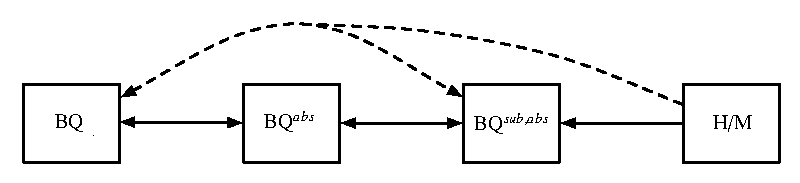
\includegraphics{images/Comparisons}
    \caption{Outline of the comparisons of \BQ, \BQa, \BQsa and Hindley/Milner. The dotted comparisons are derived from the solid ones.}
  \end{figure}
  
  \begin{dfn}
    \dfnlabel{embedded}
    We say that a type system $\Omega_1$ is embedded in a type system $\Omega_2$,
    written $\Omega_1\subseteq\Omega_2$\notation{embedded},
    if all derivations in $\Omega_1$ are derivations in $\Omega_2$.
  \end{dfn}
  \begin{thm}
    The embedding relation is reflexive and transitive.
  \end{thm}
  \begin{thm}
    \thmlabel{bq_bqa_bqsa}
    $\BQ\subseteq\BQa\subseteq\BQsa$.
  \end{thm}
  \begin{proof}[\proofthmref{bq_bqa_bqsa}]
    The embedding of \BQ in \BQa follows from \lemmaref{decabs_sdabs},
    and the embedding of \BQa in \BQsa is direct since \BQsa extends \BQa.
  \end{proof}
  \begin{dfn}
    A derivation $C;\Gamma\entailsm e:\type{T}$ is more precise than a derivation
    $C';\Gamma'\entailsm e:\type{T}'$ if $\Gamma'\subtype\Gamma$ and for all ground assignments $\phi$ and
    all ground substitutions $\theta_{\bar{\type{X}}}$ there exists a ground substitution
    $\theta_{\bar{\type{Y}}}$ such that
    $\phi\csat\theta_{\bar{\type{X}}}(C) \implies \phi\csat \theta_{\bar{\type{Y}}}(C')\textrm{ and }\phi\csat \theta_{\bar{\type{Y}}}(\type{T}')\subtype\theta_{\bar{\type{X}}}(\type{T})$, where
    $\bar{\type{X}}=\ftv(C)\cup\ftv(\type{T})\setminus\ftv(\Gamma)$ and $\bar{\type{Y}}=\ftv(C')\cup\ftv(\type{T}')\setminus\ftv(\Gamma')$.
  \end{dfn}
  \begin{thm}[Weakening]
    \thmlabel{weakening}
    If $\Gamma'\subtype\Gamma$ and $\Gamma\entailouter e:\type{S}$ in \BQsa then
    $\Gamma'\entailouter e:\type{S}'$ where $\type{S}'\subtype\type{S}$,
    and if $C;\Gamma\entailinner e:\type{T}$ in \BQsa then a more precise derivation
    $C';\Gamma'\entailsm e:\type{T}'$ can be derived.
  \end{thm}
  \begin{proof}[\proofthmref{weakening}]
  	By induction on the typing rules.
    % weakening proof - base
    \begin{indcase}{\sdbase}
      Direct since for any constant $c$, $\type{T}_c$ does not depend on the environment.
    \end{indcase}
    % weakening proof - var
    \begin{indcase}{\sdvar}
      Suppose that $\Gamma\entailsp x:\type{S}$ and $\Gamma'\subtype\Gamma$.
      By rule hypothesis $\Gamma(x)=\type{S}$
      and by definition $\Gamma'(x)=\type{S}'$ such that
      $\type{S}'\subtype\type{S}$.
      Therefore, by applying the \sdvar rule we have
      $\Gamma'\entailsp x:\type{S}'$.
    \end{indcase}
    % weakening proof - start
    \begin{indcase}{\sdstart}
      Suppose $C;\Gamma\entailsm e:\type{T}$ and $\Gamma'\subtype\Gamma$.
      By rule hypothesis, we have
      $\Gamma\entailsp e:\forall\bar{\type{X}}|C.\type{T}$ and by induction
      \begin{displaymath}
        \Gamma'\entailsp e:\forall\bar{\type{Y}}|C'.\type{T}'\quad\textrm{and}\quad
        \forall\bar{\type{Y}}|C'.\type{T}'\subtype\forall\bar{\type{X}}|C.\type{T}
      \end{displaymath}
      and after applying the \sdstart rule we have
      \begin{displaymath}
        C';\Gamma'\entailsp e:\type{T}'
      \end{displaymath}
      and by \thmref{normalform_poly}, for all
      ground assignments $\phi$ and all ground substitutions $\theta_{\bar{\type{X}}}$,
      there exists $\theta_{\bar{\type{Y}}}$ such that
      \begin{displaymath}
        \phi\csat\theta_{\bar{\type{X}}}(C) \implies
        \phi\csat\theta_{\bar{\type{Y}}}(C')\textrm{ and }
        \phi\csat\theta_{\bar{\type{Y}}}(\type{T}')\subtype\theta_{\bar{\type{X}}}(\type{T})
      \end{displaymath}
      By \lemmaref{uselesstypevariables}, it is safe to assume that
      $\bar{\type{X}}\subseteq\ftv(C)\cup\ftv(\type{T})$ and $\bar{\type{Y}}\subseteq\ftv(C')\cup\ftv(\type{T}')$.
      In addition, $\bar{\type{X}}$ and $\bar{\type{Y}}$ do not
      conflict with $\ftv(\Gamma)$ and $\ftv(\Gamma')$. Let
      \begin{displaymath}
        \begin{array}{l}
          \bar{\type{X}}' = \ftv(C)\cup\ftv(\type{T})\setminus\ftv(\Gamma)=\ftv(C)\cup\ftv(\type{T})\\
          \bar{\type{Y}}' = \ftv(C')\cup\ftv(\type{T}')\setminus\ftv(\Gamma')=\ftv(C')\cup\ftv(\type{T}')
        \end{array}
      \end{displaymath}
      %\begin{eqnarray*}
      %  \bar{\type{X}}' &=& \ftv(C)\cup\ftv(\type{T})\setminus\ftv(\Gamma)=\ftv(C)\cup\ftv(\type{T})\\
      %  \bar{\type{Y}}' &=& \ftv(C')\cup\ftv(\type{T}')\setminus\ftv(\Gamma')=\ftv(C')\cup\ftv(\type{T}')
      %\end{eqnarray*}
      and take a ground assignment $\phi$, a ground substitution $\theta_{\bar{\type{X}}'}$ and suppose
      that $\phi\csat\theta_{\bar{\type{X}}'}(C)$. Construct $\phi'$ such that
      $\phi'(\type{W})=\theta_{\bar{\type{X}}'}(\type{W})$ where
      $\type{W}\in\bar{\type{X}}'\setminus\bar{\type{X}}$ and equal to $\phi$ otherwise. By construction
      \begin{displaymath}
        \phi'\csat\theta_{\bar{\type{X}}}(C)\textrm{ and by implication }
        \phi'\csat\theta_{\bar{\type{Y}}}(C')\textrm{ and }
        \phi'\csat\theta_{\bar{\type{Y}}}(\type{T}')\subtype\theta_{\bar{\type{X}}}(\type{T})\textrm{.}
      \end{displaymath}
      Construct $\theta_{\bar{\type{Y}}'}$ such that
      $\theta_{\bar{\type{Y}}}(\type{W})=\phi'(\type{W})$ where
      $\type{W}\in\bar{\type{Y}}'\setminus\bar{\type{Y}}$ and equal to $\theta_{\bar{\type{Y}}}$
      otherwise. By construction
      \begin{displaymath}
        \phi\csat\theta_{\bar{\type{Y}}'}(C')\quad\textrm{and}\quad
        \phi\csat\theta_{\bar{\type{Y}}'}(\type{T}')\subtype\theta_{\bar{\type{X}}'}(\type{T})
      \end{displaymath}
      concluding this case.
    \end{indcase}
    % weakening proof - let
    \begin{indcase}{\sdlet}
      Suppose $C;\Gamma\entailsm \Let{x}{e_1}{e_2}:\type{T}$ and $\Gamma'\subtype\Gamma$.
      By rule hypothesis
      \begin{displaymath}
        \Gamma\entailsp e_1:\type{S}\quad\textrm{and}\quad
        C;\Gamma\cdot x:\type{S}\entailsm e_2:\type{T}
      \end{displaymath}
      and by induction $\Gamma'\entailsp e_1:\type{S}'$ where $\type{S}'\subtype\type{S}$.
      In addition $\Gamma'\cdot x:\type{S}'\subtype\Gamma\cdot x:\type{S}$, since
      $\type{S}'\subtype\type{S}$ and $x$ is a bound variable that can be freely $\alpha$-renamed.
      By induction, we therefore have $C';\Gamma'\cdot x:\type{S}'\entailsm e_2:\type{T}'$ and for all
      ground assignments $\phi$, and all ground substitutions $\theta_{\bar{\type{X}}}$ there
      exist a ground substitution $\theta_{\bar{\type{Y}}}$ such that
      \begin{displaymath}
        \phi\csat\theta_{\bar{\type{X}}}(C) \implies \phi\csat \theta_{\bar{\type{Y}}}(C')\textrm{ and }
        \phi\csat\theta_{\bar{\type{Y}}}(\type{T}')\subtype\theta_{\bar{\type{X}}}(\type{T})
      \end{displaymath}
      where $\bar{\type{X}}=\ftv(C)\cup\ftv(\type{T})\setminus\ftv(\Gamma)$ and
      $\bar{\type{Y}}=\ftv(C')\cup\ftv(\type{T}')\setminus\ftv(\Gamma')$.
      We conclude this case by applying \sdlet, yielding
      \begin{displaymath}
        C';\Gamma'\entailsm \Let{x}{e_1}{e_2}:\type{T}'\textrm{.}
      \end{displaymath}
    \end{indcase}
    % weakening proof - rec
    \begin{indcase}{\sdrec}
      Suppose
      \begin{displaymath}
        C_1\land\cdots\land C_n; \Gamma\entailsm\set{l_1=e_1,\ldots,l_n=e_n}:\set{l_1:\type{T}_1,\ldots,l_n=\type{T}_n}
      \end{displaymath}
      and $\Gamma'\subtype\Gamma$.
      If $n$ is $0$ the result is trivial, we therefore assume that it is greater or equal to $1$,
      let $i$ by an index in $[1,n]$.
      By rule hypothesis we have $C_i;\Gamma\entailsm e_i:\type{T}_i$, and by induction
      $C_i';\Gamma\entailsm e_i:\type{T}_i'$ such that, for all ground assignnments $\phi$ and all
      ground substitutions $\theta_{\bar{\type{X}}_i}$, there exists $\theta_{\bar{\type{Y}}_i}$
      such that
      \begin{displaymath}
        \phi\csat\theta_{\bar{\type{X}}_i}(C_i) \implies
        \phi\csat\theta_{\bar{\type{Y}}_i}(C_i')\textrm{ and }
        \phi\csat\theta_{\bar{\type{Y}}_i}(\type{T}_i')\subtype\theta_{\bar{\type{X}}_i}(\type{T}_i)
	  \end{displaymath}
	  where $\bar{\type{X}}_i=\ftv(C_i)\cup\ftv(\type{T}_i)\setminus\ftv(\Gamma)$ and
	  $\bar{\type{Y}}_i=\ftv(C_i')\cup\ftv(\type{T}_i')\setminus\ftv(\Gamma')$.
	  
	  It is important
	  to note that if we take $i\ne j$ then $\bar{\type{X}}_i\pound\bar{\type{X}}_j$\footnote{
	    That is $\bar{\type{X}}_i\cap\bar{\type{X}}_j=\emptyset$.}
	  and $\bar{\type{Y}}_i\pound\bar{\type{Y}}_j$.
	  Indeed, variable sharing across separate derivations occurs via the environment.
	  
	  Let $\bar{\type{X}}=\ftv\lrp{C_1\land\cdots}\cup\ftv\lrp{\set{l_1:\type{T}_1,\cdots}}\setminus\ftv(\Gamma)$ and
	  $\bar{\type{Y}}=\ftv\lrp{C_1'\land\cdots}\cup\ftv\lrp{\set{l_1:\type{T}_1',\cdots}}\setminus\ftv(\Gamma')$.
	  It is clear
	  that $\bar{\type{X}}_i\subseteq\bar{\type{X}}$ and $\bar{\type{Y}}_i\subseteq\bar{\type{Y}}$.
	  Take a ground assignment $\phi$ and ground substitution $\theta_{\bar{\type{X}}}$ such that
	  \begin{displaymath}
	    \phi\csat\theta_{\bar{\type{X}}}\lrp{C_1\land\cdots \land C_n}\textrm{.}
	  \end{displaymath}
	  Since $\ftv(C_i)=\bar{\type{X}}_i\subseteq\bar{\type{X}}$ we have
	  \begin{displaymath}
	    \phi\csat\theta_{\bar{\type{X}}_i}\lrp{C_i}
	  \end{displaymath}
	  and by implication
	  \begin{displaymath}
        \phi\csat\theta_{\bar{\type{Y}}_i}(C_i')\textrm{ and }
        \phi\csat\theta_{\bar{\type{Y}}_i}(\type{T}_i')\subtype\theta_{\bar{\type{X}}_i}(\type{T}_i)
      \end{displaymath}
      We can merge all ground substitutions into $\theta_{\bar{\type{Y}}}$ which allows us to conclude
	  \begin{displaymath}
        \phi\csat\theta_{\bar{\type{Y}}}(C_1\land\cdots\land C_n)\textrm{ and }
        \phi\csat\theta_{\bar{\type{Y}}}(\type{T}_i')\subtype\theta_{\bar{\type{X}}}(\type{T}_i)
      \end{displaymath}
      and by \srec and \csub
	  \begin{displaymath}
        \phi\csat\theta_{\bar{\type{Y}}}(\set{l_1:\type{T}_1',\cdots,l_n:\type{T}_n'})\subtype\theta_{\bar{\type{X}}}(\set{l_1:\type{T}_1,\cdots,l_n:\type{T}_n})
      \end{displaymath}
      concluding this case.
    \end{indcase}
    % weakening proof - sel
    \begin{indcase}{\sdsel}
      Suppose $C\land\type{T}\subtype\set{l:\type{W}};\Gamma\entailsm e.l:\type{W}$
      and $\Gamma'\subtype\Gamma$.
      By rule hypothesis
      \begin{displaymath}
        C;\Gamma\entailsm e:\type{T}\quad\textrm{and}\quad
        \type{W}\textrm{ is fresh}\textrm{.}
      \end{displaymath}
      By induction $C';\Gamma'\entailsm e:\type{T}'$ and for all
      ground assignments $\phi$ and all ground substitutions $\theta_{\bar{\type{X}}}$, there
      exist a ground substitution $\theta_{\bar{\type{Y}}}$ such that
      \begin{displaymath}
        \phi\csat\theta_{\bar{\type{X}}}(C) \implies \phi\csat \theta_{\bar{\type{Y}}}(C')\textrm{ and }\phi\csat \theta_{\bar{\type{Y}}}(\type{T}')\subtype\theta_{\bar{\type{X}}}(\type{T})
      \end{displaymath}
      where $\bar{\type{X}}=\ftv(C)\cup\ftv(\type{T})\setminus\ftv(\Gamma)$ and
      $\bar{\type{Y}}=\ftv(C')\cup\ftv(\type{T}')\setminus\ftv(\Gamma')$.
      Applying the \sdsel rule yields
      \begin{displaymath}
        C'\land\type{T}'\subtype\set{l:\type{W}};\Gamma'\entailsm e.l:\type{W}
      \end{displaymath}
      since $\type{W}$ is fresh.
      Let
      \begin{displaymath}
        \begin{array}{l}
          \bar{\type{X}}' =\ftv\lrp{C\land\type{T}\subtype\set{l:\type{W}}}\cup\ftv(\type{T})\setminus\ftv(\Gamma)=
            \bar{\type{X}}\cup\type{W} \\
          \bar{\type{Y}}' =\ftv\lrp{C'\land\type{T}'\subtype\set{l:\type{W}}}\cup\ftv(\type{T}')\setminus\ftv(\Gamma')=
            \bar{\type{Y}}\cup\type{W}
        \end{array}
      \end{displaymath}
      and take an arbitrary ground substitution $\theta_{\bar{\type{X}}'}$ and a ground assignment $\phi$
      satisfying $\theta_{\bar{\type{X}}'}(C\land\type{T}\subtype\set{l:\type{W}})$.
      Take the ground assignment
      $\phi'$ similar to $\phi$ in every position except for
      $\phi'(\type{W})=\theta_{\bar{\type{X}}'}(\type{W})$. By construction,
      $\phi'\csat \theta_{\bar{\type{X}}}(C)$ and by implication
      $\phi'\csat \theta_{\bar{\type{Y}}}(C')$ and
      $\phi'\csat \theta_{\bar{\type{Y}}}(\type{T}')\subtype\theta_{\bar{\type{X}}}(\type{T})$,
      for some ground substitution $\theta_{\bar{\type{Y}}}$.
      Since $\type{W}$ is fresh, it does not appear in $C$, $C'$, $\type{T}$ nor in $\type{T}'$.
      Therefore
      \begin{displaymath}
        \phi\csat \theta_{\bar{\type{Y}}'}(C') \quad\textrm{and}\quad
        \phi\csat \theta_{\bar{\type{Y}}'}(\type{T}')\subtype\theta_{\bar{\type{X}}'}(\type{T})
      \end{displaymath}
      where we select $\theta_{\bar{\type{Y}}'}$ such that
      $\theta_{\bar{\type{Y}}'}(\type{W})=\theta_{\bar{\type{X}}'}(\type{W})$.
      
      By interpretation of $\phi\csat\theta_{\bar{\type{X}}'}(C\land\type{T}\subtype\set{l:\type{W}})$
      \begin{displaymath}
        \phi\csat\theta_{\bar{\type{X}}'}(C)\quad\textrm{and}\quad
        \phi\csat\theta_{\bar{\type{X}}'}(\type{T}\subtype\set{l:\type{W}})\textrm{.}
      \end{displaymath}
      Pushing the ground substitution we have
      $\phi\csat\theta_{\bar{\type{X}}'}(\type{T})\subtype\theta_{\bar{\type{X}}'}(\set{l:\type{W}})$.
      As $\theta_{\bar{\type{X}}'}(\type{W})=\theta_{\bar{\type{Y}}'}(\type{W})$ and
      $\phi\csat \theta_{\bar{\type{Y}}'}(\type{T}')\subtype\theta_{\bar{\type{X}}'}(\type{T})$
      we can derive using \cand
      \begin{displaymath}
        \phi\csat\theta_{\bar{\type{Y}}'}(C'\land\type{T}'\set{l:\type{W}})\textrm{.}
      \end{displaymath}
      Finally, $\phi\csat\theta_{\bar{\type{Y}}'}(\type{W})\subtype\theta_{\bar{\type{X}}'}(\type{W})$
      since $\theta_{\bar{\type{Y}}'}(\type{W})=\theta_{\bar{\type{X}}'}(\type{W})$,
      concluding this case.
    \end{indcase}
    % weakening proof - abs
    \begin{indcase}{\decabs}
      Suppose $C;\Gamma\entailsm \lambda x.e:\type{T}_1\fun\type{T}_2$
      and $\Gamma'\subtype\Gamma$. By rule hypothesis
      \begin{displaymath}
        C;\Gamma\cdot x:\forall\emptyset|\true.\type{T}_1\entailsm e:\type{T}_2
      \end{displaymath}
      and $\Gamma'\cdot x:\forall\emptyset|\true.\type{T}_1\subtype\Gamma\cdot x:\forall\emptyset|\true.\type{T}_1$
      as $x$ is bound in $e$ and therefore does not conflict with $\Gamma'$. By induction
      \begin{equation}
        \label{eq:w_sdabs_1}
        C';\Gamma'\cdot x:\forall\emptyset|\true.\type{T}_1\entailsm e:\type{T}_2'
      \end{equation}
      and for all
      ground assignments $\phi$ and all ground substitutions $\theta_{\bar{\type{X}}}$, there
      exists a ground substitution $\theta_{\bar{\type{Y}}}$ such that
      \begin{displaymath}
        \phi\csat \theta_{\bar{\type{X}}}(C) \implies \phi\csat \theta_{\bar{\type{Y}}}(C')\textrm{ and }\phi\csat \theta_{\bar{\type{Y}}}(\type{T}_2')\subtype\theta_{\bar{\type{X}}}(\type{T}_2)
      \end{displaymath}
      where
      \begin{displaymath}
        \begin{array}{l}
          \bar{\type{X}} = \ftv(C)\cup\ftv(\type{T}_2)\setminus\ftv\lrp{\Gamma\cdot x:\forall\emptyset|\true.\type{T}_1}
            =\ftv(C)\cup\ftv(\type{T}_2)\setminus\ftv(\Gamma)\cup\ftv(\type{T}_1)\\
          \bar{\type{Y}} = \ftv(C')\cup\ftv(\type{T}_2')\setminus\ftv\lrp{\Gamma\cdot x:\forall\emptyset|\true.\type{T}_1}
            =\ftv(C')\cup\ftv(\type{T}_2')\setminus\ftv(\Gamma')\cup\ftv(\type{T}_1)
        \end{array}
      \end{displaymath}
      Applying \sdabs to \eqref{eq:w_sdabs_1} yields
      \begin{displaymath}
        C';\Gamma'\entailsm \lambda x.e:\type{T}_1\fun\type{T}_2'\textrm{.}
      \end{displaymath}
      Let
      \begin{displaymath}
        \begin{array}{l}
          \bar{\type{X}}' = \ftv\lrp{C}\cup\ftv(\type{T}_1\fun\type{T}_2)\setminus\ftv(\Gamma)
            =\bar{\type{X}}\cup\ftv(\type{T}_1)\\
          \bar{\type{Y}}' = \ftv\lrp{C'}\cup\ftv(\type{T}_1\fun\type{T}_2')\setminus\ftv(\Gamma')
            =\bar{\type{Y}}\cup\ftv(\type{T}_1)
        \end{array}
      \end{displaymath}
      Let $\type{W}\in\ftv(\type{T}_1)$ and
      take two arbitrary ground substitution $\theta_{\bar{\type{X}}'}$,
      $\theta_{\bar{\type{Y}}'}$ such that
      $\theta_{\bar{\type{X}}'}(\type{W})=\theta_{\bar{\type{Y}}'}(\type{W})$ and a ground assignment $\phi$
      satisfying $\theta_{\bar{\type{X}}'}(C)$. Take $\phi'$ equal to $\phi$ except for
      $\phi'(\type{W})=\phi\lrp{\theta_{\bar{\type{X}}'}(\type{W})}$ and
      $\phi'(\type{W})=\phi\lrp{\theta_{\bar{\type{Y}}'}(\type{W})}$.
      By construction, $\phi'$ satisfies $\theta_{\bar{\type{X}}}(C)$, and by implication
      \begin{displaymath}
        \phi'\csat \theta_{\bar{\type{Y}}}(C') \quad\textrm{and}\quad
        \phi'\csat \theta_{\bar{\type{Y}}}(\type{T}_2')\subtype\theta_{\bar{\type{X}}}(\type{T}_2)
      \end{displaymath}
      thus $\phi\csat\theta_{\bar{\type{Y}}'}(C')$ and
      $\phi\csat\theta_{\bar{\type{Y}}'}(\type{T}_1\fun\type{T}_2')\subtype\theta_{\bar{\type{X}}'}(\type{T}_1\fun\type{T}_2)$ concluding this case.
    \end{indcase}
    % weakening proof - app
    \begin{indcase}{\sdapp}
      Suppose
      \begin{displaymath}
        \underbrace{C_1\land C_2\land\type{T}_1\subtype\type{X}\fun\type{Y}\land\type{T}_2\subtype\type{X}}_C;\Gamma\entailsm e_1\ e_2:\type{Y}
      \end{displaymath}
      and $\Gamma'\subtype\Gamma$. By rule hypothesis
      \begin{displaymath}
        C_1;\Gamma\entailsm e_1:\type{T}_1\quad\textrm{and}\quad
        C_2;\Gamma\entailsm e_2:\type{T}_2\quad\textrm{and }
        \type{X},\type{Y}\textrm{ are fresh.}
      \end{displaymath}
      By induction
      \begin{displaymath}
        C_1';\Gamma'\entailsm e_1:\type{T}_1'\quad\textrm{and}\quad
        C_2';\Gamma'\entailsm e_2:\type{T}_2'
      \end{displaymath}
      and for all
      ground assignments $\phi$ and all ground substitutions $\theta_{\bar{\type{X}}_1}$, $\theta_{\bar{\type{X}}_2}$,
      there exists ground substitutions $\theta_{\bar{\type{Y}}_1}$, $\theta_{\bar{\type{Y}}_2}$ such that
      \begin{eqnarray}
        \phi\csat\theta_{\bar{\type{X}}_1}(C_1) \implies
        \phi\csat\theta_{\bar{\type{Y}}_1}(C_1')\textrm{ and }
        \phi\csat\theta_{\bar{\type{Y}}_1}(\type{T}_1')\subtype\theta_{\bar{\type{X}}_1}(\type{T}_1)\nonumber\\
        \phi\csat\theta_{\bar{\type{X}}_2}(C_2) \implies
        \phi\csat\theta_{\bar{\type{Y}}_2}(C_2')\textrm{ and }
        \phi\csat\theta_{\bar{\type{Y}}_2}(\type{T}_2')\subtype\theta_{\bar{\type{X}}_2}(\type{T}_2)\nonumber
      \end{eqnarray}
      where $\bar{\type{X}_1}=\ftv(C_1)\cup\ftv(\type{T}_1)\setminus\ftv(\Gamma)$,
      $\bar{\type{X}_2}=\ftv(C_2)\cup\ftv(\type{T}_2)\setminus\ftv(\Gamma)$,
      $\bar{\type{Y}_1}=\ftv(C_1')\cup\ftv(\type{T}_1')\setminus\ftv(\Gamma')$,
      $\bar{\type{Y}_2}=\ftv(C_2')\cup\ftv(\type{T}_2')\setminus\ftv(\Gamma')$.
      We have $\bar{\type{X}}_1\pound\bar{\type{X}}_2$ and $\bar{\type{Y}}_1\pound\bar{\type{Y}}_2$
      as explained in the \sdrec case. Applying the \sdapp gives
      \begin{displaymath}
        \underbrace{C_1'\land C_2'\land \type{T}_1'\subtype\type{X}\fun\type{Y}\land\type{T}_2'\subtype\type{X}}_{C'};\Gamma'\entailsm e_1\ e_2:\type{Y}
      \end{displaymath}
      Let
      \begin{displaymath}
        \begin{array}{l}
          \bar{\type{X}} = \ftv(C)\cup\ftv(\type{Y})\setminus\ftv(\Gamma)=\bar{\type{X}_1}\cup\bar{\type{X}_2}\cup\set{\type{X},\type{Y}}\\
          \bar{\type{Y}} = \ftv(C')\cup\ftv(\type{Y})\setminus\ftv(\Gamma')=\bar{\type{Y}_1}\cup\bar{\type{Y}_2}\cup\set{\type{X},\type{Y}}
        \end{array}
      \end{displaymath}
      Take a ground assignment $\phi$ and a ground substitution $\theta_{\bar{\type{X}}}$ such that
      $\theta_{\bar{\type{X}}}(C)$ is satisfied. By interpetation
      \begin{displaymath}
        \phi\csat\theta_{\bar{\type{X}}}(C_1)\quad
        \phi\csat\theta_{\bar{\type{X}}}(C_2)\quad
        \phi\csat\theta_{\bar{\type{X}}}(\type{T}_1\subtype\type{X}\fun\type{Y})\quad
        \phi\csat\theta_{\bar{\type{X}}}(\type{T}_2\subtype\type{X})\textrm{.}
      \end{displaymath}
      We can restrict the domain of $\theta_{\bar{\type{X}}}$ to $\theta_{\bar{\type{X}}_1}$
      and $\theta_{\bar{\type{X}}_2}$ and we have
      \begin{displaymath}
        \phi\csat\theta_{\bar{\type{X}}_1}(C_1)\quad
        \phi\csat\theta_{\bar{\type{X}}_2}(C_2)
      \end{displaymath}
      and by implication
      \begin{displaymath}
        \phi\csat\theta_{\bar{\type{Y}}_1}(C_1')\quad
        \phi\csat\theta_{\bar{\type{Y}}_1}(\type{T}_1')\subtype\theta_{\bar{\type{X}}_1}(\type{T}_1)\quad
        \phi\csat\theta_{\bar{\type{Y}}_2}(C_2')\quad
        \phi\csat\theta_{\bar{\type{Y}}_1}(\type{T}_2')\subtype\theta_{\bar{\type{X}}_1}(\type{T}_2)
      \end{displaymath}
      Construct $\theta_{\bar{\type{Y}}}$ as the union of $\theta_{\bar{\type{Y}}_1}$ and $\theta_{\bar{\type{Y}}_2}$
      such that $\theta_{\bar{\type{Y}}}(\type{X})=\theta_{\bar{\type{X}}}(\type{X})$ and
      $\theta_{\bar{\type{Y}}}(\type{Y})=\theta_{\bar{\type{X}}}(\type{Y})$. We have
      \begin{displaymath}
        \phi\csat\theta_{\bar{\type{Y}}}(C_1')\quad
        \phi\csat\theta_{\bar{\type{Y}}}\lrp{\type{T}_1'\subtype\type{X}\fun\type{Y}}\quad
        \phi\csat\theta_{\bar{\type{Y}}}(C_2')\quad
        \phi\csat\theta_{\bar{\type{Y}}}\lrp{\type{T}_2'\subtype\type{Y}}
      \end{displaymath}
      which concludes this case.
    \end{indcase}
    % weakening proof - fin
    \begin{indcase}{\sdfin}
      Suppose $\Gamma\entailsp e:\forall\bar{\type{X}}|C.\type{T}$ and $\Gamma'\subtype\Gamma$.
      By rule hypothesis
      \begin{displaymath}
        C;\Gamma\entailsm e:\type{T} \quad
        \bar{\type{X}}=\ftv(\type{T})\cup\ftv(C)\setminus\ftv(\Gamma) \quad
        \cissat C\textrm{.}
      \end{displaymath}
      By induction $C';\Gamma'\entailsm e:\type{T}'$ and for all ground assignments $\phi$
      \begin{displaymath}
        \phi\csat\theta_{\bar{\type{X}}}(C) \implies
        \phi\csat\theta_{\bar{\type{Y}}}(C')\textrm{ and }
        \phi\csat\theta_{\bar{\type{Y}}}(\type{T}')\subtype\theta_{\bar{\type{X}}}(\type{T})
      \end{displaymath}
      where $\bar{\type{Y}}=\ftv(\type{T}')\cup\ftv(C')\setminus\ftv(\Gamma')$. Since $C$ is satisfiable,
      there exists a ground assignment $\phi$ and a ground substitution $\theta_{\ftv(C)}$
      such that $\phi\csat\theta_{\ftv(C)}(C)$. From this, one can construct a ground assignment
      $\phi'$ and a ground substitution $\theta_{\bar{\type{X}}}$ such that
      $\phi(\theta_{\ftv(C)}(C))=\phi'(\theta_{\bar{\type{X}}}(C))$ and therefore
      $\phi'\csat\theta_{\bar{\type{X}}}(C)$.
      By implication $\phi'\csat\theta_{\bar{\type{Y}}}(C')$ and doing the same
      `backward conversion' shows that $C'$ is satisfiable. By applying the \sdfin rule
      we get
      \begin{displaymath}
        \Gamma'\entailsp e:\forall\bar{\type{Y}}|C'.\type{T}'
      \end{displaymath}
      and we are going to show that
      $\forall\bar{\type{Y}}|C'.\type{T}'\subtype\forall\bar{\type{X}}|C.\type{T}$. Fix
      a ground assignment $\phi$ and let $\type{T}^\star\in\sinterp{\forall\bar{\type{X}}|C.\type{T}}$.
      By definition of \dfnref{upclosure} and \dfnref{poly_interpretation}
      \begin{displaymath}
        \phi\lrp{\theta_{\bar{\type{X}}}(\type{T})}\subtype\type{T}^\star\quad\textrm{and}\quad
        \phi\csat\theta_{\bar{\type{X}}}(C)
      \end{displaymath}
      by implication
      \begin{displaymath}
        \phi\csat\theta_{\bar{\type{Y}}}(C')\quad\textrm{and}\quad
        \phi\csat\theta_{\bar{\type{Y}}}(\type{T}')\subtype\theta_{\bar{\type{X}}}(\type{T})
      \end{displaymath}
      for some ground substitution $\theta_{\bar{\type{Y}}}$. By transitivity of the subtyping
      relation \thmref{subtyping_mono}
      \begin{displaymath}
        \phi\csat\theta_{\bar{\type{Y}}}(\type{T}')\subtype\type{T}^\star
      \end{displaymath}
      which is equivalent to $\phi\lrp{\theta_{\bar{\type{Y}}}(\type{T}')}\subtype\phi\lrp{\type{T}^\star}$,
      and $\phi\lrp{\type{T}^\star}=\type{T}^\star$ since $\type{T}^\star$ is a ground type.
      Therefore
      \begin{displaymath}
        \type{T}^\star\in\sinterp{\forall\bar{\type{Y}}|C'.\type{T}'}
      \end{displaymath}
      proving that $\sinterp{\forall\bar{\type{X}}|C.\type{T}}\subseteq\sinterp{\forall\bar{\type{Y}}|C'.\type{T}'}$.
      By definition \dfnref{poly_subtype} $\forall\bar{\type{Y}}|C'.\type{T}'\subtype\forall\bar{\type{X}}|C.\type{T}$,
      concluding this case.
    \end{indcase}
    % weakening proof - sub
    \begin{indcase}{\decsub}
      Immediate.
    \end{indcase}
  \end{proof}
  \begin{cor}
    \corlabel{weakening_cor}
    The weakening theorem applies to \BQ and \BQa.
  \end{cor}
  \begin{dfn}
    We define an expression's context as an expression with a single hole
    \begin{displaymath}
      E \eqg \Hole
        \mid \lambda x.E
        \mid \eapp{E_1}{e_2}
        \mid \eapp{e_1}{E_2}
        \mid \elet{x}{E_1}{e_2}
        \mid \elet{x}{e_1}{E_2}
        \mid \set{l_1:e_1,\ldots,l_k:E_k,\ldots,l_n:e_n}
        \mid \esel{E}{l}\textrm{.}
    \end{displaymath}
  \end{dfn}
  \begin{thm}
    \thmlabel{bqsubabs_replacebyvar}
    Let $\Gamma\entailsp e:\type{S}_1$, if $\Gamma\entailsp E[e]:\type{S}_2$ then
    $\Gamma\cdot x:\type{S}_1\entailsp E[x]:\type{S}_2$, and similarly if
    $\Gamma\entailsp E[e]:\type{T}_2$ then
    $\Gamma\cdot x:\type{S}_1\entailsp E[x]:\type{T}_2$ with
    $x\notin\dom(\Gamma)$ and is not bound in $E$.
  \end{thm}
  \begin{proof}[\proofthmref{bqsubabs_replacebyvar}]
    Direct since the typing rules do not inspect an expression's shape
    once the expression has been typed.
  \end{proof}
  \begin{cor}
    \corlabel{bqsubabs_dependent}
    If $\Gamma\entailsp e:\type{S}_1$, $\Gamma\entailsp E[e]:\type{S}_2$ and
    $\Gamma\entailsp e':\type{S}_1'$ with $\type{S}_1'\subtype\type{S}_1$ then
    $\Gamma\entailsp E[e']:\type{S}_2'$ with $\type{S}_2'\subtype\type{S}_2$.
    
    If $C_1;\Gamma\entailsp e:\type{T}_1$, $C_2;\Gamma\entailsp E[e]:\type{T}_2$ and
    a more precise derivation $C_1'\Gamma\entailsp e':\type{T}_1'$ then
    $C_2';\Gamma\entailsp E[e']:\type{T}_2'$ is a more precise derivation.
  \end{cor}
  \begin{proof}[\proofcorref{bqsubabs_dependent}]
    Follows from \thmref{weakening} and \thmref{bqsubabs_replacebyvar}.
  \end{proof}
  \begin{thm}
    \thmlabel{bqsubabs_bqabs}
    If $\Gamma\entailouter e:\type{S}$ is derivable in \BQsa then
    $\Gamma\entailouter e:\type{S}'$ is derivable in \BQa with $\type{S}'\subtype\type{S}$.
  \end{thm}
  \begin{proof}[\proofthmref{bqsubabs_bqabs}]
    By full induction on the number of uses of the \decsub rule in a derivation.
    
    We suppose that if there are $n$ or fewer uses of the \decsub rule we have a derivation in
    \BQa deriving $\type{S}'$ such that $\type{S}'\subtype\type{S}$. Consider a derivation
    with $n+1$ uses of the \decsub rule. Pick one use of the \decsub rule dividing the derivation into
    two sub-derivations $\Delta_1$ and $\Delta_2$ deriving $\type{S}_1$, $\type{S}_2$
    in which the \decsub rule is used $n$ times of fewer.
    Inductively, we have two sub-derivations $\Delta_1'$ and $\Delta_2'$ in
    \BQa deriving $\type{S}_1'$, $\type{S}_2'$ with
    $\type{S}_1'\subtype\type{S}_1$ and $\type{S}_2'\subtype\type{S}_2$.
    If $\Delta_2'$ is not an empty derivation (in which case we can conclude immediately),
    the first rule is either \sdstart or \sdlet. We can conclude using \corref{bqsubabs_dependent}
    for the first case and weakening \thmref{weakening} for the second.
  \end{proof}
  \begin{figure}[ht]
    \centering
    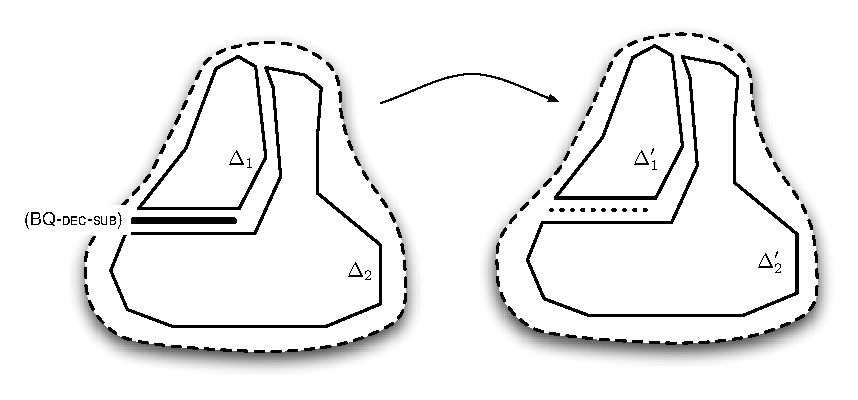
\includegraphics{images/BQsa_to_BQa}
    \caption{Comparison of derivations in \BQa and \BQa.}
  \end{figure}
  \begin{thm}
    \thmlabel{bqabs_map}
    If $\Gamma\entailsp e:\forall\bar{\type{X}}|C.\type{T}$ is derivable in \BQa then
    for all maps $\psi$ such that $\psi(\Gamma')=\Gamma$,
    $\Gamma'\entailsp e:\forall\bar{\type{Y}}|C'.\type{T}'$ is derivable
    and for all substitutions $\theta_{\bar{\type{X}}}$ there exists $\theta_{\bar{\type{Y}}}$
    with $\psi({\theta_{\bar{\type{Y}}}(C')})=\theta_{\bar{\type{X}}}(C)$,
    $\psi({\theta_{\bar{\type{Y}}}(\type{T}')})=\theta_{\bar{\type{X}}}(\type{T})$.
    
    In addition, if $C;\Gamma\entailsm e:\type{T}$ is
    derivable in \BQa then for all maps $\psi$ such that $\psi(\Gamma')=\Gamma$, the
    derivation $C';\Gamma'\entailsm e:\type{T}'$
    is derivable with $\psi(C')=C$ and $\psi(\type{T}')=\type{T}$.
  \end{thm}
  \begin{proof}[\proofthmref{bqabs_map}]
  	By induction on the typing rules.
    % proof - base
    \begin{indcase}{\sdbase}
      Immediate since a constant's type does not depend on the environment.
    \end{indcase}
    % proof - var
    \begin{indcase}{\sdvar}
      Suppose $\Gamma\entailsp x:\type{S}$ and take $\psi$ and $\Gamma'$ such that $\psi(\Gamma')=\Gamma$.
      By rule hypothesis $\Gamma(x)=\type{S}$ and therefore $\psi(\Gamma')(x)=\type{S}$ which allows
      us to conclude this case.
    \end{indcase}
    % proof - start
    \begin{indcase}{\sdstart}
      For the purpose of the proof, we highlight the silent substitution implied
      by the \sdstart rule yielding
      \begin{mathpar}
        \infrule{\sdstart}{
          \Gamma\entailsp e:\forall\bar{\type{X}}|C.\type{T}
        }{\theta_{\bar{\type{X}}}(C);\Gamma\entailsm e:\theta_{\bar{\type{X}}}(\type{T})}\textrm{.}
      \end{mathpar}
      Suppose $\theta_{\bar{\type{X}}}(C);\Gamma\entailsm e:\theta_{\bar{\type{X}}}(\type{T})$
      and take $\psi$ and $\Gamma'$ such that $\psi(\Gamma')=\Gamma$.
      By rule hypothesis $\Gamma\entailsp e:\forall\bar{\type{X}}|C.\type{T}$ and by induction
      $\Gamma'\entailsp e:\forall\bar{\type{Y}}|C'.\type{T}'$ and
      for all substitutions $\theta_{\bar{\type{X}}}$ there exists $\theta_{\bar{\type{Y}}}$ such that
      $\psi(\theta_{\bar{\type{Y}}}(C'))=\theta_{\bar{\type{X}}}(C)$ and
      $\psi(\theta_{\bar{\type{Y}}}(\type{T}'))=\theta_{\bar{\type{X}}}(\type{T})$.
      We can therefore apply the \sdstart rule and conclude.
    \end{indcase}
    % proof - let
    \begin{indcase}{\sdlet, \sdrec, \sdsel, \decabs, \sdapp}
      Immediate.
    \end{indcase}
    % proof - fin
    \begin{indcase}{\sdfin}
      Suppose $\Gamma\entailsp e:\forall\bar{\type{X}}|C.\type{T}$
      and take $\psi$ and $\Gamma'$ such that $\psi(\Gamma')=\Gamma$. By rule hypothesis
      $C;\Gamma\entailsm e:\type{T}$, $\bar{\type{X}}=\ftv(\type{T})\cup\ftv(C)\setminus\ftv(\Gamma)$
      and $\cissat C$. By induction $C';\Gamma'\entailsp e:\type{T}'$ is derivable
      with $\psi(C')=C$ and $\psi(\type{T}')=\type{T}$. Since $C$ is satifiable, $C'$ is also satisfiable
      (there exists a ground assignment $\phi$ such that $\phi\csat C$ thus $\phi\circ\psi\csat C'$).
      Now, let $\bar{\type{Y}}=\ftv(\type{T}')\cup\ftv(C')\setminus\ftv(\Gamma')$ and take a substitution
      $\theta_{\bar{\type{X}}}$. We are going to show that there exists a substitution $\theta_{\bar{\type{Y}}}$
      satisfying $\psi(\theta_{\bar{\type{Y}}}(C'))=\theta_{\bar{\type{X}}}(C)$ and
      $\psi(\theta_{\bar{\type{Y}}}(\type{T}'))=\theta_{\bar{\type{X}}}(\type{T})$.
      Indeed $\bar{\type{X}}=\ftv\lrp{\psi(\bar{\type{Y}})}$ as derived below
      \begin{eqnarray*}
        \bar{\type{X}} &=& \ftv(\type{T})\cup\ftv(C)\setminus\ftv(\Gamma) \\
          &=& \ftv(\psi(\type{T}'))\cup\ftv(\psi(C'))\setminus\ftv(\psi(\Gamma')) \\
          &=& \ftv(\psi(\ftv(\type{T}')))\cup\ftv(\psi(\ftv(C')))\setminus\ftv(\psi(\ftv(\Gamma'))) \\
          &=& \ftv\lrp{\psi\lrp{\ftv(\type{T}')\cup\ftv(C')\setminus\ftv(\Gamma')}} \\
          &=& \ftv\lrp{\psi(\bar{\type{Y}})}\textrm{.}
      \end{eqnarray*}
      We can conclude by using the \sdfin rule.
    \end{indcase}
  \end{proof}
  \begin{cor}
    \corlabel{bqabs_bq}
    If $\Gamma\entailsp e:\forall\bar{\type{X}}|C.\type{T}$ is derivable in \BQa then
    there exists a map $\psi$ such that
    $\Gamma'\entailsp e:\forall\bar{\type{Y}}|C'.\type{T}'$ is derivable in \BQ
    and for all substitutions $\theta_{\bar{\type{X}}}$ there exists $\theta_{\bar{\type{Y}}}$
    with $\psi({\theta_{\bar{\type{Y}}}(C')})=\theta_{\bar{\type{X}}}(C)$,
    $\psi({\theta_{\bar{\type{Y}}}(\type{T}')})=\theta_{\bar{\type{X}}}(\type{T})$.
    
    In addition, if $C;\Gamma\entailsm e:\type{T}$ is
    derivable in \BQa then
    there exists a map $\psi$ such that
    $C';\Gamma'\entailsm e:\type{T}'$
    is derivable in \BQ with $\psi(\Gamma')=\Gamma$, $\psi(C')=C$ and $\psi(\type{T}')=\type{T}$.
  \end{cor}
  \begin{proof}[\proofcorref{bqabs_bq}]
    Follows from \thmref{bqabs_map}. When using the \sdabs rule one can select an environment
    with a type variable for the \BQ derivation and map it to the type chosen in the \BQa derivation.
  \end{proof}
  \begin{cor}
    \corlabel{bqsubabs_bq}
    If $\Gamma\entailouter e:\type{S}$ is derivable in \BQsa then
    $\Gamma\entailouter e:\type{S}'$ is derivable in \BQ with $\type{S}'\subtype\type{S}$.
  \end{cor}
  \begin{proof}[\proofcorref{bqsubabs_bq}]
    Follows from \corref{bqabs_bq} and \thmref{bqsubabs_bqabs}.
  \end{proof}
  
  \chapter{Conservative Extension of Hindley/Milner}
  In this section, we are going to show that our type system is a conservative
  extension of Hindley/Milner's type system. For this, we compare Hindley/Milner to
  \BQsa and show that Hindley/Milner's derivation can be matched.
  
  \section{Survey of Hindley/Milner}
  Expressions in Hindley/Milner are generated by the following grammar.
  \begin{displaymath}
    e \eqg c
      \mid x
      \mid \lambda x.
      \mid \eapp{e_1}{e_2}
      \mid \elet{x}{e_1}{e_2}{.}
  \end{displaymath}
  We have constants $c$ (which we suppose are the same as in the BQ family), variables,
  anonymous functions and let polymorphism.
  Monomorphic types consist of base types, type variables and functional
  types.
  \begin{displaymath}
    \type{T} \eqg \type{B}
             \mid \type{X}
             \mid \type{T}_1\fun\type{T}_2{.}
  \end{displaymath}
  We further assume that the set of type variables is the same as in the BQ family.
  One can observe that the expressions and monomorphic types in the BQ family
  extend those of Hindley/Milner, which can be formalized by the following theorem.
  \begin{thm}
    \thmlabel{mlexp_is_bqexp}
    Let $e$ be an expression in Hindley/Milner, then $e$ is an expression in the BQ family. Similarly,
    if $\type{T}$ is a monomorphic Hindley/Milner type, then it is also a type in the BQ family.
  \end{thm}
  \begin{proof}
    \thmref{mlexp_is_bqexp}
    Follows directly from the definition of expressions and monomorphic types.
  \end{proof}
  Hindley/Milner polymorphic types are either a monomorphic type or a generalized type.
  \begin{displaymath}
    \type{S} \eqg \type{T}
             \mid \forall\bar{\type{X}}.\type{T}{.}
  \end{displaymath}
  In the BQ family, polymorphic types are separate from monomorphic types and are constrained.
  We thus convert Hindley/Milner polymorphic types to the BQ family.
  \begin{dfn}
    Let $\mltobq{\cdot}$ denote a type conversion function from Hindley/Milner to the BQ family
    defined by
    \begin{mathpar}
      \mltobq{\type{T}} = \forall\emptyset|\true.\type{T} \and
      \mltobq{\forall\bar{\type{X}}.\type{T}} = \forall\bar{\type{\type{X}}}|\true.\type{T}
    \end{mathpar}
    and we lift this definition to environments
    \begin{displaymath}
      \mltobq{\Gamma} = \coll{x:\mltobq{\type{S}}}{x:\type{S}\in\Gamma}\textrm{.}
    \end{displaymath}
  \end{dfn}
  \begin{lemma}
    \lemmalabel{mlexp_ftvconversion}
    Let $\type{S}$ be a Hindley/Milner polymorphic type, then
    $\ftv\lrp{\type{S}}=\ftv\lrp{\mltobq{\type{S}}}$.
  \end{lemma}
  \begin{proof}[\prooflemmaref{mlexp_ftvconversion}]
    Immediate.
  \end{proof}
  
  \subsection{Hindley/Milner Typing Rules}
  We repeat for clarity Hindley/Milner's type inference. The rules we consider are adapted
  from Pottier and R\'emy \cite{pottier-remy-emlti} but the original presentation of
  Damas and Milner \cite{damasmilner:principal-type-schemes} is very close.
  \notation{entailsml}
  \begin{mathpar}
    \infrule{\mlbase}{
      \Base(c) = \type{T}_c
    }{\Gamma\entailsml c:\type{T}_c} \and
    \infrule{\mlvar}{
      \Gamma(x) = \type{S}
    }{\Gamma\entailsml x:\type{S}} \and
    \infrule{\mlabs}{
      \Gamma\cdot x:\type{T}_1\entailsml e:\type{T}_2
    }{\Gamma\entailsml\lambda x.e:\type{T}_1\fun\type{T}_2} \and
    \infrule{\mlapp}{
      \Gamma\entailsml e_1:\type{T}_1\fun\type{T}_2 \and
      \Gamma\entailsml e_2:\type{T}_1
    }{\Gamma\entailsml e_1 \ e_2 : \type{T}_2} \and
    \infrule{\mllet}{
      \Gamma\entailsml e_1:\type{S} \and
      \Gamma\cdot x:\type{S}\entailsml e_2:\type{T}
    }{\Gamma\entailsml \elet{x}{e_1}{e_2}:\type{T}} \and
    \infrule{\mlgen}{
      \Gamma\entailsml e:\type{T} \and \bar{\type{X}} \pound \ftv(\Gamma)
    }{\Gamma\entailsml e:\forall\bar{\type{X}}.\type{T}} \and
    \infrule{\mlinst}{
      \Gamma\entailsml e:\forall\bar{\type{X}}.\type{T}
    }{\Gamma\entailsml e:\type{T}}
  \end{mathpar}
  We add the base rule \mlbase to introduce constants and their associated
  types in Hindley/Milner thus comparing coherently the BQ family to Hindley/Milner.
  
  \section{Comparison}
  We now compare our type system with Hindley/Milner. We show that
  every type derivation in Hindley/Milner is also derivable in \BQsa
  \thmref{bqsa_ml} and later give a direct comparison between our algorithmic presentation \BQ
  and Hindley/Milner \thmref{bq_ml}.
  
  \begin{thm}
    \thmlabel{bqsa_ml}
    If $\Gamma\entailsml e:\type{S}$ then $\mltobq{\Gamma}\entailsp e:\mltobq{\type{S}}$ in \BQsa.
  \end{thm}
  \begin{proof}[\proofthmref{bq_ml}]
    By induction on the Hindley/Milner typing rules.
    \begin{indcase}{\mlbase}
      Immediate since $\mltobq{\Base(c)}=\forall\emptyset|\true.\Base(c)$.
    \end{indcase}
    \begin{indcase}{\mlvar}
      Suppose $\Gamma\entailsml x:\type{S}$. By rule hypothesis $\Gamma(x)=\type{S}$
      and by definition $\mltobq{\Gamma}(x)=\mltobq{\type{S}}$. By applying the
      \sdvar rule we have $\mltobq{\Gamma}\entailsp x:\mltobq{\type{S}}$.
    \end{indcase}
    \begin{indcase}{\mlabs}
      Suppose $\Gamma\entailsml \lambda x.e:\type{T}_1\fun\type{T}_2$. By rule hypothesis
      $\Gamma\cdot x:\type{T}_1\entailsml e:\type{T}_2$ and by induction
      \begin{displaymath}
        \underbrace{\mltobq{\Gamma\cdot x:\type{T}_1}}_{\mltobq{\Gamma}\cdot x:\forall\emptyset|\true.\type{T}_1}\entailsp
        e:\underbrace{\mltobq{\type{T}_2}}_{\forall\emptyset|\true.\type{T}_2}
      \end{displaymath}
      we can derive
      \begin{mathpar}
        \inferrule*[Left=\sdfin]{
          \inferrule*[Left=\decabs]{
            \inferrule*[Left=\sdstart]{
              \mltobq{\Gamma}\cdot x:\forall\emptyset|\true.\type{T}_1\entailsp e:\forall\emptyset|\true.\type{T}_2
            }{\true;\mltobq{\Gamma}\cdot x:\forall\emptyset|\true.\type{T}_1\entailsm e:\type{T}_2}
          }{\true;\mltobq{\Gamma}\entailsm \lambda x.e:\type{T}_1\fun\type{T}_2} \and
          \cissat \true
        }{\mltobq{\Gamma}\entailsp \lambda x.e:\forall\bar{\type{X}}|\true.\type{T}_1\fun\type{T}_2}
      \end{mathpar}
      where $\bar{\type{X}}=\ftv\lrp{\type{T}_1\fun\type{T}_2}\cup\ftv(\true)\setminus\ftv\lrp{\mltobq{\Gamma}}$.
      By lemma \lemmaref{schemesmallerset}
      \begin{displaymath}
        \forall\bar{\type{X}}|\true.\type{T}_1\fun\type{T}_2\subtype
        \forall\emptyset|\true.\type{T}_1\fun\type{T}_2=
        \mltobq{\type{T}_1\fun\type{T}_2}
      \end{displaymath}
      and we can conclude by applying the \decsub rule.
    \end{indcase}
    \begin{indcase}{\mlapp}
      Suppose $\Gamma\entailsml e_1\ e_2:\type{T}_2$. By rule hypothesis
      $\Gamma\entailsml e_1:\type{T}_1\fun\type{T}_2$ and
      $\Gamma\entailsml e_2:\type{T}_1$. By induction
      \begin{mathpar}
        \mltobq{\Gamma}\entailsp
        e_1:\underbrace{\mltobq{\type{T}_1\fun\type{T}_2}}_{\forall\emptyset|\true.\type{T}_1\fun\type{T}_2} \and
        \mltobq{\Gamma}\entailsp
        e_2:\underbrace{\mltobq{\type{T}_1}}_{\forall\emptyset|\true.\type{T}_1}
      \end{mathpar}
      and we can derive
      \begin{mathpar}
        \inferrule*[Left=\sdfin]{
          \inferrule*[Left=\sdapp]{
            \inferrule*[Left=\sdstart]{
              \mltobq{\Gamma}\entailsp e_1:\forall\emptyset|\true.\type{T}_1\fun\type{T}_2
            }{\true;\mltobq{\Gamma}\entailsm e_1:\type{T}_1\fun\type{T}_2} \and
            \inferrule*[Right=\sdstart]{
              \mltobq{\Gamma}\entailsp e_2:\forall\emptyset|\true.\type{T}_1
            }{\true;\mltobq{\Gamma}\entailsm e_2:\type{T}_1}
          }{\ensuremath{\overbrace{\true\land\true\land\type{T}_1\fun\type{T}_2\subtype\type{X}\fun\type{Y}\land\type{T}_1\subtype\type{X}}^{C}};\mltobq{\Gamma}\entailsm e_1\ e_2:\type{Y}}\and
          \cissat C
        }{\mltobq{\Gamma}\entailsp e_1\ e_2:\forall\bar{\type{X}}|C.\type{Y}}
      \end{mathpar}
      where $\bar{\type{X}}=\ftv(\type{Y})\cup\ftv(C)\setminus\ftv\lrp{\mltobq{\Gamma}}$.
      As $\forall\bar{\type{X}}|C.\type{Y}\subtype\forall\emptyset|\true.\type{T}_2=\mltobq{\type{T}_2}$,
      we can conclude by applying the \decsub rule.
    \end{indcase}
    \begin{indcase}{\mllet}
      Suppose $\Gamma\entailsml\elet{x}{e_1}{e_2}:\type{T}$. By rule hypothesis $\Gamma\entailsml e_1:\type{S}$
      and $\Gamma\cdot x:\type{S}\entailsml e_2:\type{T}$. By induction
      \begin{mathpar}
        \mltobq{\Gamma}\entailsp e_1:\mltobq{\type{S}} \and
        \underbrace{\mltobq{\Gamma\cdot x:\type{S}}}_{\mltobq{\Gamma}\cdot x:\mltobq{\type{S}}}\entailsp
        e_2:\underbrace{\mltobq{\type{T}}}_{\forall\emptyset|\true.\type{T}}
      \end{mathpar}
      we can derive
      \begin{mathpar}
        \inferrule*[Left=\sdfin]{
          \inferrule*[Left=\sdlet]{
            \mltobq{\Gamma}\entailsp e_1:\mltobq{\type{S}} \and
            \inferrule*[Right=\sdstart]{
              \mltobq{\Gamma}\cdot x:\mltobq{\type{S}}\entailsp e_2:\forall\emptyset|\true.\type{T}
            }{\true;\mltobq{\Gamma}\cdot x:\mltobq{\type{S}}\entailsm e_2:\type{T}}
          }{\true;\mltobq{\Gamma}\entailsm\elet{x}{e_1}{e_2}:\type{T}}\and
          \cissat \true
        }{\mltobq{\Gamma}\entailsp\elet{x}{e_1}{e_2}:\forall\bar{\type{X}}|\true.\type{T}}
      \end{mathpar}
      where $\bar{\type{X}}=\ftv\lrp{\type{T}}\cup\ftv(\true)\setminus\ftv\lrp{\mltobq{\Gamma}}$.
      By lemma \lemmaref{schemesmallerset}
      \begin{displaymath}
        \forall\bar{\type{X}}|\true.\type{T}\subtype
        \forall\emptyset|\true.\type{T}=\mltobq{\type{T}}
      \end{displaymath}
      and we can conclude by applying the \decsub rule.
    \end{indcase}
    \begin{indcase}{\mlgen}
      Suppose $\Gamma\entailsml e:\forall\bar{\type{X}}.\type{T}$. Without loss of generality,
      we suppose that the conversion of $\forall\bar{\type{X}}.\type{T}$ does not mention
      type variables vacuously \lemmaref{uselesstypevariables}. By rule hypothesis
      $\Gamma\entailsml e:\type{T}$ and $\bar{\type{X}}\pound\ftv(\Gamma)$ and by induction
      $\mltobq{\Gamma}\entailsp e:\mltobq{\type{T}}$. We can derive
      \begin{mathpar}
        \inferrule*[Left=\sdfin]{
          \inferrule*[Left=\sdstart]{
            \mltobq{\Gamma}\entailsp e:\mltobq{\type{T}}
          }{\true;\mltobq{\Gamma}\entailsm e:\type{T}}\and
          \cissat \true
        }{\mltobq{\Gamma}\entailsm e:\forall\bar{\type{Y}}|\true.\type{T}}
      \end{mathpar}
      where $\bar{\type{Y}}=\ftv\lrp{\type{T}}\cup\ftv(\true)\setminus\ftv\lrp{\mltobq{\Gamma}}$.
      By \lemmaref{mlexp_ftvconversion} we know that $\bar{\type{X}}\subseteq\bar{\type{Y}}$
      and by \lemmaref{schemesmallerset}
      \begin{displaymath}
        \forall\bar{\type{Y}}|\true.\type{T}\subtype
        \forall\bar{\type{X}}|\true.\type{T}=
        \mltobq{\forall\bar{\type{X}}.\type{T}}
      \end{displaymath}
      which allows us to conclude by applying the \decsub rule.
    \end{indcase}
    \begin{indcase}{\mlinst}
      Immediate since $\mltobq{\forall\bar{\type{X}}.\type{T}}\subtype\mltobq{\type{T}}$.
    \end{indcase}
  \end{proof}
  \begin{thm}
    \thmlabel{bq_ml}
    If $\Gamma\entailsml e:\type{S}$ then $\mltobq{\Gamma}\entailsp e:\type{S}'$ in \BQ with
    $\type{S}'\subtype\mltobq{\type{S}}$.
  \end{thm}
  \begin{proof}[\proofthmref{bq_ml}]
    Follows directly from \corref{bqsubabs_bq} and \thmref{bqsa_ml}.
  \end{proof}
  
  \chapter{More on Constraints}
  \section{Efficiency of Constraint Solving}
  We now concentrate on the efficiency of constraint solving.
  Building upon previous algebraic results \cite{benke93,pratt96satisfiability,tiuryn92},
  we show that constraint satisfiability in presence of positive subtyping is PTIME-complete.
  Benke \cite{benke93}
  showed that satisfiability of inequalities in Helly posets \dfnref{helly} is decidable in PTIME.
  To reuse this result, our analysis defines the type poset $\Types$ as a term algebra of functions
  and records constructed from atomic types \dfnref{atomictypes} and show that the term algebra
  construction preserves the Helly property.
    
  We begin our analysis by defining fences, distances, disks and
  the Helly property. Quilliot \cite{appofhelly} introduced these definitions;
  Nevermann/Rival \cite{holes} and Benke \cite{benke93} later reformulated them.
  Intuitively, a fence is an oscillating path within a poset, each
  oscillation corresponding to a shift in the direction the path takes  
  along the links in the poset.
  The distance between two elements in a
  poset is the number of oscillations in the smallest fence that links  
  the two elements.
  A disk of a given size $\mathbf{n}$ around an element $\type{T}$ is the set of
  elements at distance less than $\mathbf{n}$ from $\type{T}$.
  
  Introducing positive functional subtyping over an arbitrary poset  
  preserves all structural properties. In effect,
  positive functional subtyping lifts
  the subtyping relation of the poset but does not alter its shape. In
  particular, introducing positive functional subtyping preserves the  
  Helly property.
  Contra-variant functional subtyping, in
  comparison, greatly modifies the shape of posets (\figref{positiveversusstd}). Hoang and
  Mitchell \cite{hoang:lower-bounds} studied the latter
  case and showed that satisfiability of inequalities in that context can
  be PSPACE-hard.
  
  \begin{figure}[ht]
    \centering
    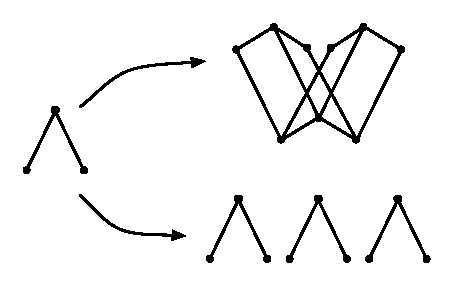
\includegraphics{images/positiveversusstd}
    \caption{Positive Subtyping vs. Contra-variant Subtyping -- one arrow posets are shown.}
    \figlabel{positiveversusstd}
  \end{figure}
  
  Since our base type poset is trivial and positive functional  
  subtyping simply lifts the underlying subtyping
  relation, we need to introduce
  non-trivial subtyping. We have chosen to do so using records and show  
  that
  record subtyping preserves the Helly property. This approach differs  
  from Hoang and Mitchell \cite{hoang:lower-bounds}, who consider a
  complex base type poset
  and introduce contra-variant functional subtyping. Finally, note that
  our results would hold over any base type poset that has the Helly  
  property, which includes lattices and trees.
  \begin{dfn}
    \notation{upfence}
    \notation{downfence}
    An up-fence of length $n$ from $\type{T}_1$ to $\type{T}_2$ in $P$,
    written $F_P^+(\type{T}_1, \type{T}_2)$, is a set
    $\set{\type{U}_0,\ldots,\type{U}_n}$ such that $\type{T}_1=\type{U}_0$
    and $\type{T}_2=\type{U}_n$ such that
    $\type{U}_{2i}\subtype\type{U}_{2i+1}\rsubtype\type{U}_{2i+2}$.
    A down fence $F_P^-(\type{T}_1, \type{T}_2)$ is defined equivalently with
    $\type{U}_{2i}\rsubtype\type{U}_{2i+1}\subtype\type{U}_{2i+2}$.
  \end{dfn}
  An up-fence between $\type{T}_1$ and $\type{T}_2$ could be a down-fence from $\type{T}_2$
  to $\type{T}_1$. The direction of a fence is not inherent to its structure, but rather a
  point of view. In the next section, we explore precisely this duality.
  \begin{figure}[ht]
    \begin{minipage}[b]{0.5\linewidth}
      \centering
      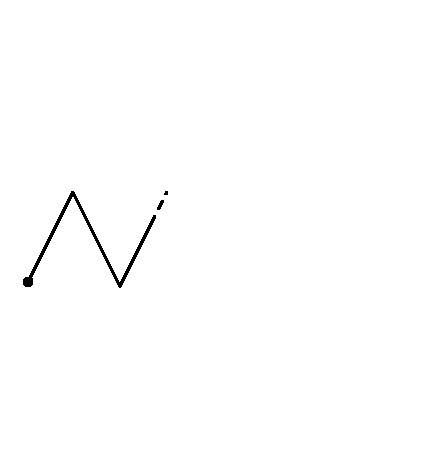
\includegraphics{images/up-fence_medium}
      \caption{An up-fence.}
    \end{minipage}
    \begin{minipage}[b]{0.5\linewidth}
      \centering
      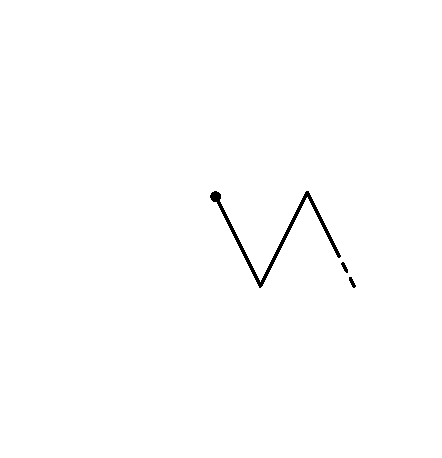
\includegraphics{images/down-fence_medium}
      \caption{A down-fence.}
    \end{minipage}
  \end{figure}
  \begin{dfn}
    \notation{updistance}
    \notation{downdistance}
    The up-distance $d_P^+(\type{T}_1,\type{T}_2)$ of two elements in a poset $P$ is the smallest
    integer $n$ such that there exists an up-fence of length $n$ from $\type{T}_1$ to $\type{T}_2$.
    The down-distance is defined dually. Finally, the distance $\type{T}_1$ to $\type{T}_2$
    is defined as
    \begin{displaymath}
      d_P(\type{T}_1,\type{T}_2)=\lrp{d_P^+(\type{T}_1,\type{T}_2), d_P^-(\type{T}_1,\type{T}_2)}\textrm{.}
    \end{displaymath}
  \end{dfn}
  \begin{dfn}
    \notation{disk}
    A disk of center $\type{T}$ and of radius $\mathbf{n}=(n^+,n^-)$ in P is the set
    \begin{displaymath}
      D_P\lrp{\type{T}, \mathbf{n}} = \coll{\type{U}\in P}{d_P\lrp{\type{T},\type{U}}\le\mathbf{n}}
    \end{displaymath}
    that is, the set of all $\type{U}$ satisfying the two inequatlities
    $d_P^+(\type{T},\type{U})\le n^+$ and $d_P^-(\type{T},\type{U})\le n^-$.
  \end{dfn}
  \begin{dfn}
    \dfnlabel{helly}
    An ordered set satisfies the two-disk property (also known as the Helly property)
    if, for every family $\mathcal{D}$ of disks,
    \begin{displaymath}
      \bigcap\mathcal{D}\neq\emptyset
    \end{displaymath}
    whenever $D_1\cap D_2\neq\emptyset$ for each $D_1$, $D_2$ in $\mathcal{D}$.
  \end{dfn}
  
  \subsubsection{Poset with Arrow}
  We consider a partially ordered set (or poset) which we extend by adding positive
  subtyping. As mentioned earlier, Hoang and Mitchell \cite{hoang:lower-bounds}
  consider this case in depth for contra-variant subtyping.
  
  \begin{dfn}
    Let $\poset{P,\subtype_P}$ be a partially ordered set. We denote by $P^\fun$\notation{pfun} the term
    algebra over $(P,\fun)$. It is partially ordered by extending the $\subtype_P$ using
    the \sfun rule.
  \end{dfn}
  We define an equivalence relation that partitions types of $P^\fun$
  based on their arrow structure. This relation
  requires invariant types to be equal and considers co-variant types
  as equivalent.
  \begin{dfn}
    We define the relation $\equivt$\notation{eq} by
    \begin{mathpar}
      \infrule{\eqbase}{
        \type{T}_1\in P\and
        \type{T}_2\in P
      }{\type{T}_1\equivt\type{T}_2} \and
      \infrule{\eqarrow}{
        \type{T}_2\equivt\type{T}_2'
      }{\type{T}_1\fun\type{T}_2\equivt\type{T}_1\fun\type{T}_2'}
    \end{mathpar}
    and we say that $\type{T}_1$ has the same arrow structure as $\type{T}_2$ whenever
    $\type{T}_1\equivt\type{T}_2$.
  \end{dfn}
  The following theorem captures the properties of the $\equivt$ relation.
  \begin{thm}
    $\equivt$ is an equivalence relation. We denote by $\class{\type{T}}_\equivt$\notation{eqclass} the
    equivalence class of $\type{T}$ under $\equivt$.
  \end{thm}
  We now capture the equality of invariant types under the equivalence relation.
  \begin{thm}
    \thmlabel{eqclassextractsame}
    If $\type{T}_1\fun\type{T}_1'$ and $\type{T}_2\fun\type{T}_2'$ are elements of $\class{\type{T}}_\equivt$,
    then $\type{T}_1=\type{T}_2$.
  \end{thm}
  To exploit the equivalence relation and link it with the subtyping relation,
  we define an extraction function which selects the co-variant portion of a type.
  \begin{dfn}
    We define the function \extract\ by
    \begin{mathpar}
      \infrule{\exbase}{
        \type{T}\in P
      }{\extract(\type{T}) = \type{T}} \and
      \infrule{\exarrow}{
        \extract(\type{T}_2) = \type{T}_2'
      }{\extract(\type{T}_1\fun\type{T}_2) = \type{T}_2'}
    \end{mathpar}
    which extracts the lower right leaf of a type.
  \end{dfn}
  The extraction function maps types in $P^\fun$ to types in $P$.
  \begin{thm}
    The range of \extract\ is $P$.
  \end{thm}
  The invariance of the argument type of a functional type makes
  subtyping in $P^\fun$ reducible to subtyping in $P$, and by extension
  each equivalence class $\class{\type{T}}_\equivt$ is isomorphic to $P$
  \thmref{eqclassisomorphic}.
  \begin{thm}
    \thmlabel{extract_subtype}
    If $\type{T}_1$ and $\type{T}_2$ are elements of $\class{\type{T}}_\equivt$ then
    $\type{T}_1\subtype\type{T}_2$ if and only if $\extract(\type{T}_1)\subtype\extract(\type{T}_2)$.
  \end{thm}
  \begin{proof}[\proofthmref{extract_subtype}]
    By induction on $\type{T}_2$.
    \begin{indcase}{$\type{T}_2\in P$}
       By normal form \thmref{normalform_mono}, $\type{T}_1\in P$ and we can conclude
       since $\extract(\type{T}_1)=\type{T}_1$ and $\extract(\type{T}_2)=\type{T}_2$.
    \end{indcase}
    \begin{indcase}{$\type{T}_2=\type{T}_{12}\fun\type{T}_2'$}
      \begin{innerindcase}{$\Rightarrow$}
        We suppose that $\type{T}_1\subtype\type{T}_2$.
        By normal form \thmref{normalform_mono}, $\type{T}_1=\type{T}_{12}\fun\type{T}_1'$ and
        $\type{T}_1'\subtype\type{T}_2'$. By induction $\extract(\type{T}_1')\subtype\extract(\type{T}_2')$
        and thus $\extract(\type{T}_1)\subtype\extract(\type{T}_2)$.
      \end{innerindcase}
      \begin{innerindcase}{$\Leftarrow$}
        We suppose that $\extract(\type{T}_1)\subtype\extract(\type{T}_2)$ and we conclude
        using \thmref{eqclassextractsame}.
      \end{innerindcase}
    \end{indcase}
  \end{proof}
  \begin{thm}
    \thmlabel{eqclassisomorphic}
    $\class{\type{T}}_\equivt$ is isomorphic to $P$.
  \end{thm}
  \begin{proof}[\proofthmref{eqclassisomorphic}]
    Let $\type{T}$ be in $P^\fun$. We suppose that it is not in $P$ since this case is trivial.
    Define the map $\varphi(\type{U})=\extract(\type{\type{U}})$ between $\class{\type{T}}_\equivt$
    and $P$. We have shown that
    \begin{displaymath}
      \varphi(\type{U}_1)\subtype\varphi(\type{U}_2) \iff \type{U}_1 \subtype \type{U}_2
    \end{displaymath}
    and since $\varphi$ is one-to-one and onto, $\varphi$ is in fact an isomorphism.
  \end{proof}
  \begin{cor}
    $P^\fun$ is partitioned by $\equivt$ into isomorphic copies of $P$.
  \end{cor}
  \begin{thm}
    \thmlabel{pfunhelly}
    If $P$ satisfies the Helly property so does $P^\fun$.
  \end{thm}
  \begin{proof}[\proofthmref{pfunhelly}]
    Immediate since $P^\fun$ is partitioned into isomorphic copies of $P$.
  \end{proof}
  
  \subsection{Poset with Records}
  In this section, we prove that the structural subtyping introduced by records
  preserves the Helly property. We build a term algebra for records \dfnref{recorcdtermalgebra}
  and give an inductive proof.
  \begin{dfn}
    \dfnlabel{recorcdtermalgebra}
    \notation{prec}
    Let $\poset{P,\subtype_P}$ be a partially ordered set. We define
    \begin{eqnarray*}
      P^{\rec(0)} &=& P \\
      P^{\rec(k+1)} &=& P^{\rec(k)}\cup
        \bigcup_{\set{l_1,\ldots,l_n}\subset\Labels}\set{l_1:P^{\rec(k)}, \ldots, l_n:P^{\rec(k)}} \\
      P^\rec &=& \bigcup_{k\ge 0}P^{\rec(k)}
    \end{eqnarray*}
    and we extend the partial ordering $\subtype_P$ using the \srec rule.
  \end{dfn}
  Given two types, the up-distance between them is at most 2 since every type
  is a subtype of top, and by symmetry their down-distance is at most 3.
  \begin{thm}
    \thmlabel{maxupmaxdown}
    The maximal up-distance in $P^\rec$ is $2$, and the maximal down-distance is $3$.
  \end{thm}
  \begin{proof}[\proofthmref{maxupmaxdown}]
    Follows from the presence of $\top$.
  \end{proof}
  Based on the previous observation and on the definition of distance,
  we can give a simpler presentation of disks in $P^\rec$.
  \begin{thm}
    \thmlabel{disksshapeinprec}
    Disks $D_{P^\rec}\lrp{\type{T}, \mathbf{n}}$ have the shapes outlined in \figref{disks}.
  \end{thm}
  \begin{figure}[ht]
    \centering
    \begin{tabular}[c]{l|lll}
      $\mathbf{n}$ & 0 & 1 & 2 \\
      \hline
      0  & $\set{\type{T}}$ & $\set{\type{T}}$ & $\set{\type{T}}$ \\
      1  & $\set{\type{T}}$ & $\set{\type{T}}$ & $\downclosure{\type{T}}$ \\
      2  & $\set{\type{T}}$ & $\upclosure{\type{T}}$ & $\upclosure{\type{T}}\cup\downclosure{\type{T}}$ \\
      3  & $\set{\type{T}}$ & $\upclosure{\type{T}}$ & $P^\rec$
    \end{tabular}
    \caption{Disks in $P^\rec$.}
    \figlabel{disks}
  \end{figure}
  \begin{proof}[\proofthmref{disksshapeinprec}]
    We show three cases, the others are similar.
    \begin{eqnarray*}
      D_{P^\rec}\lrp{\type{T}, (1, 1)}
        &=& \coll{\type{U}}{d^+(\type{T},\type{U})\le 1\land d^-(\type{T},\type{U})\le 1}\\
        &=& \coll{\type{U}}{\type{T}\subtype\type{U}\land\type{U}\subtype\type{T}}\\
        &=& \set{\type{T}}\\
        &&\\
      D_{P^\rec}\lrp{\type{T}, (2, 1)}
        &=& \coll{\type{U}}{d^+(\type{T},\type{U})\le 2\land d^-(\type{T},\type{U})\le 1}\\
        &=& \coll{\type{U}}{\exists\type{U}':\type{T}\subtype\type{U}'\land\type{U}\subtype\type{U}'\land\type{U}\subtype\type{T}}\\
        &=& \downclosure{\type{T}}\\
        &&\\
      D_{P^\rec}\lrp{\type{T}, (2, 2)}
        &=& \coll{\type{U}}{d^+(\type{T},\type{U})\le 2\land d^-(\type{T},\type{U})\le 2}\\
        &=& \coll{\type{U}}{\exists\type{U}',\type{U}'':\type{T}\subtype\type{U}'\land\type{U}\subtype\type{U}'\land\type{U}''\subtype\type{T}\land\type{U}''\subtype\type{U}}\\
        &=& \upclosure{\type{T}}\cup\downclosure{\type{T}}
    \end{eqnarray*}
  \end{proof}
  \begin{thm}
    \thmlabel{prechelly}
    If $P$ satisfies the Helly property so does $P^\rec$.
  \end{thm}
  \begin{proof}[\proofthmref{prechelly}]
    We suppose that $P$ satisfies the Helly property, and we prove that $P^\rec$
    satisfies it by induction on $P^\rec$.
    \begin{indcase}{$P^{\rec(0)}$}
      Immediate.
    \end{indcase}
    \begin{indcase}{$P^{\rec(k+1)}$}
      By induction, $P^\rec(k)$ satisfies the Helly property.
      We only consider disks of radius $(2,1)$ since the others contain $\top$ or intersect trivially.
      Take a family of disks
      $\mathcal{D}$ such that for each $D_1,D_2\in\mathcal{D}$ we have $D_1\cap D_2\neq\emptyset$.
      For each pair of disk $D_1=\downclosure\type{T}_1$ and $D_2=\downclosure\type{T}_2$ we
      have $\type{T}_{12}\subtype\type{T}_1$ and $\type{T}_{12}\subtype\type{T}_2$. The two types
      $\type{T}_1$, $\type{T}_2$ must either be both in $P^{\rec(k)}$ or both in $P^{\rec(k+1)}$,
      because of the subtyping relation. The former case being trivial, we concentrate on the latter.
      By normal form \thmref{normalform_mono} $\type{T}_{12}$ contains at least the union of
      $\type{T}_{1}$ and $\type{T}_{2}$'s labels. Since these observations have been made on arbitrary
      disks, we can construct a type $\type{T}_\bot$ of the union of all the $\type{T}_i$'s labels.
      Depth subtyping can be approached with a similar reasoning, if $\type{T}_i$ and $\type{T}_j$
      have intersecting labels then we have a common subtype.
      
      Note that when considering a whole expression, the number of labels is finite
      and we thus need not worry about infinite family of disks.
    \end{indcase}
  \end{proof}
  
  \subsection{Poset with Arrow and Record}
  We now combine the previous results and use the $\fun$ and $\rec$ constructions to
  iteratively construct a type poset \dfnref{funrecconstruction}. We then show that
  this iterative construction produces the type poset $\Types$ \thmref{afunreceqtypes}
  and can therefore conclude that our types satisfy the Helly property.
  \begin{dfn}
    \dfnlabel{funrecconstruction}
    \notation{pfunrec}
    Let $\poset{P,\subtype_P}$ be a partially ordered set. We define
    \begin{eqnarray*}
      P^{\fun,\rec(0)} &=& P \\
      P^{\fun,\rec(k+1)} &=& \lrp{\lrp{P^{\fun,\rec(k)}}^\fun}^\rec \\
      P^{\fun,\rec} &=& \bigcup_{k\ge 0}P^{\fun,\rec(k)}\textrm{.}
    \end{eqnarray*}
  \end{dfn}
  \begin{dfn}
    \dfnlabel{atomictypes}
    Let $\ATypes$ denote the set of atomic types defined as the union of base types,
    type variables $\TVars$ and the top type.
  \end{dfn}
  \begin{thm}
    \thmlabel{afunreceqtypes}
    $\ATypes^{\fun,\rec}=\Types$.
  \end{thm}
  \begin{proof}[\proofthmref{afunreceqtypes}]
    By double inclusion.
    \begin{indcase}{$\subseteq$}
      Direct since $\Types$ is the term algebra from which $\ATypes$ is constructed.
    \end{indcase}
    \begin{indcase}{$\supseteq$}
      By induction on $\type{T}\in\Types$.
      \begin{innerindcase}{$\top$, $\basetype$, $\type{X}$}
        Immediate since these types are in $\ATypes$.
      \end{innerindcase}
      \begin{innerindcase}{$\type{T}_1\fun\type{T}_2$}
        By induction $\type{T}_1\in\ATypes^{\fun,\rec}$ and $\type{T}_2\in\ATypes^{\fun,\rec}$.
        Since $\type{T}_1$ and $\type{T}_2$ are finite terms, there exists $n_1$ and $n_2$ such
        that $\type{T}_1\in\ATypes^{\fun,\rec(n_1)}$ and $\type{T}_2\in\ATypes^{\fun,\rec(n_2)}$.
        Let $n=\max(n_1,n_2)$, we have $\type{T}_1\in\ATypes^{\fun,\rec(n)}$ and $\type{T}_2\in\ATypes^{\fun,\rec(n)}$,
        and we show that $\type{T}=\type{T}_1\fun\type{T}_2\in\ATypes^{\fun,\rec(n+1)}$
        \begin{eqnarray*}
          \ATypes^{\fun,\rec(n+1)} &=& \lrp{\lrp{P^{\fun,\rec(n)}}^\fun}^\rec \\
            &\supseteq& \lrp{P^{\fun,\rec(n)}}^\fun \\
            &\supseteq& P^{\fun,\rec(n)}\fun P^{\fun,\rec(n)}
        \end{eqnarray*}
        since $\type{T}\in P^{\fun,\rec(n)}\fun P^{\fun,\rec(n)}$ we have by inclusion that
        $\type{T}\in\ATypes^{\fun,\rec(n+1)}$ and a fortiori
        $\type{T}\in\ATypes^{\fun,\rec}$ concluding this case.
      \end{innerindcase}
      \begin{innerindcase}{$\set{\vec{l} : \vec{\type{T}_l}}$}
        Exact same reasoning as for the previous case.
      \end{innerindcase}
    \end{indcase}
  \end{proof}
  \begin{thm}
    \thmlabel{atypeshelly}
    $\ATypes$ satisfies the Helly property.
  \end{thm}
  \begin{proof}[\proofthmref{atypeshelly}]
    Immediate since $\ATypes$ is a tree.
  \end{proof}
  \begin{cor}
    \corlabel{typeshelly}
    $\Types$ satisfies the Helly property.
  \end{cor}
  \begin{proof}[\proofcorref{typeshelly}]
    $\ATypes^{\fun,\rec}$ is a Helly poset since $\ATypes$ satisfies the Helly property \thmref{atypeshelly}
    and $\fun$, $\rec$ are Helly property preserving \thmref{pfunhelly}, \thmref{prechelly}.
    In addition, we have shown that $\ATypes^{\fun,\rec}=\Types$ \thmref{afunreceqtypes}.
  \end{proof}
  \begin{cor}
    Satisfiability of a system of inequalities in $\Types$ is decidable in PTIME.
  \end{cor}
  \begin{proof}[\proofcorref{typeshelly}]
    Follows from Benke \cite{benke93}.
  \end{proof}
  
  \section{Satisfiability of Constraints}
  Benke \cite{benke93} showed that a Helly poset is satisfiable if and only if
  it is weakly satisfiable \dfnref{weaksat} and distance consistent \dfnref{distanceconsistent}.
  Since our types form a Helly poset, we can apply this result with minor changes to our work.
  In this section, we describe weak satisfiability and
  the distance consistency inference system Benke \cite{benke93}
  defined and discuss its use in our type inference system.
  
  We consider a subset of the constraint language presented earlier, namely subtyping constraints
  ($\type{T}_1\subtype\type{T}_2$) and logical conjunction ($C_1\land C_2$). Constraints can therefore
  be seen as a set of subtyping constraints. Removing the
  $\true$ predicate does not modify the satisfiability
  of constraints, and the $\false$ predicate cannot appear in a satisfiable set of constraints.
  In addition, the existential quantifier can be floated out.
  Finally, we solve constraints in $\GTypes$, eliminating universally quantified type variables.
  Since we are concerned with satisfiability \dfnref{cissat}, this restriction does not impact
  the expressiveness of our type system.
  
  \begin{dfn}
    \dfnlabel{weaksat}
    A constraint $C$ is weakly satisfiable if the constraint $C'$ obtained by replacing
    subtyping constraints by equality constraints and mapping base types to a constant $\star$
    is satisfiable.
  \end{dfn}
  For the sake of weak satisfiability, record equality compares common labels only and requires
  one record type's labels to be a subset of the other's record type.
  Weak satisfiability can be seen as a shape consistency and is a necessary condition to
  satisfiability. Weak satisfiability can be verified using unification and is
  therefore PTIME-complete \cite{linearunification, efficientunification}.
  
  \subsection{Distance Consistency}
  We define a two-place predicate
  $C\entailsdc d^\epsilon(\type{T}_1\subtype\type{T}_2)\le n$\notation{entailsdc} which can be
  read as ``if $C$ is satisfiable, the $\epsilon$-distance between $\type{T}_1$ and $\type{T}_2$
  must be less than or equal to $n$'' where $\epsilon$ is either $+$ for up-distance or $-$ for down-distance.
  \begin{mathpar}
    \infrule{\dcax}{
      \type{T}_1\subtype\type{T}_2\in C
    }{C\entailsdc d^+(\type{T}_1,\type{T}_2)\le 1} \and
    \infrule{\dcsymm}{
      C\entailsdc d^\epsilon(\type{T}_1,\type{T}_2)\le n
    }{C\entailsdc d^{\epsilon(-1)^n}(\type{T}_2,\type{T}_1)\le n} \and
    \infrule{\dcdual}{
      C\entailsdc d^{\epsilon}(\type{T}_1,\type{T}_2)\le n
    }{C\entailsdc d^{-\epsilon}(\type{T}_1,\type{T}_2)\le n+1} \and
    \infrule{\dcjoin}{
      C\entailsdc d^{\epsilon}(\type{T}_1,\type{T}_2)\le n\and
      C\entailsdc d^{\epsilon(-1)^{n-1}}(\type{T}_2,\type{T}_3)\le m\and
      \ensuremath{k = \left\{\begin{array}{cl}m & n=0 \\ n & m=0 \\ n+m-1 & \textrm{otherwise}\end{array}\right.}
    }{C\entailsdc d^{\epsilon}(\type{T}_1,\type{T}_3)\le k} \and
    \infrule{\dcsubfun}{
      C\entailsdc d^{\epsilon}(\type{T}_1\fun\type{T}_2,\type{T}_1'\fun\type{T}_2')\le n\and
      n\in D_\epsilon\textrm{ where }D_+=\set{1}\textrm{ and }D_-=\set{1,2}
    }{C\entailsdc d^{+/-}(\type{T}_1,\type{T}_1')=0 \and C\entailsdc d^{\epsilon}(\type{T}_2\type{T}_2')\le n} \and
    \infrule{\dcsubrec}{
      C\entailsdc d^{\epsilon}(\set{\vec{l}_-:\vec{\type{T}}_-},\set{\vec{l}_+:\vec{\type{T}}_+})\le n
    }{C\entailsdc d^{\epsilon}(\type{T}_-^l,\type{T}_+^l)\le n \and l\in\bar{l}_\epsilon}
  \end{mathpar}
  The axiomatic rule \dcax transforms a subtyping constraint into an up-distance constraint.
  If $\type{T}_1$ is a subtype of $\type{T}_2$, then we can draw a unit up-fence between them.
  The symmetry rule \dcsymm is a combination of two cases. In the first case, if the up-distance
  (respectively down-distance) between $\type{T}_1$ and $\type{T}_2$ is even, the fence
  joining $\type{T}_1$ and $\type{T}_2$ is symmetrical; therefore we can constrain the up-distance
  (respectively down-distance) between $\type{T}_2$ and $\type{T}_1$. \figref{dcsymmeven} illustrates
  this graphical symmetry. In the second case, if the up-distance
  (respectively down-distance) between $\type{T}_1$ and $\type{T}_2$ is odd, the fence's edges
  are in two different directions. Consequently, we constrain the down-distance (respectively
  up-distance). We illustrate this case in \figref{dcsymmodd}.
  \begin{figure}[ht]
    \centering
    \begin{minipage}[b]{0.4\linewidth}
      \centering
      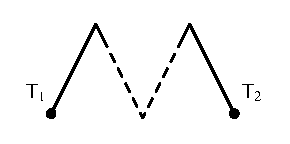
\includegraphics{images/dcsymm_even}
      \caption{\dcsymm with an even distance.
        $d^+(\type{T}_1,\type{T}_2)$ can be reversed to derive $d^+(\type{T}_2,\type{T}_1)$.}
      \figlabel{dcsymmeven}
    \end{minipage}
    \begin{minipage}[b]{0.2\linewidth}
      \centering
      \hole
    \end{minipage}
    \begin{minipage}[b]{0.4\linewidth}
      \centering
      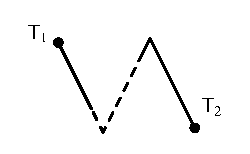
\includegraphics{images/dcsymm_odd}
      \caption{\dcsymm with an odd distance.
        $d^-(\type{T}_1,\type{T}_2)$ can be reversed to derive $d^+(\type{T}_2,\type{T}_1)$.}
      \figlabel{dcsymmodd}
    \end{minipage}
  \end{figure}
  The dual rule \dcdual constrains the inverse distance between two types. Knowing that $\type{T}_2$
  is reachable from $\type{T}_1$, using an $n$ distance fence, we can derive that an
  $n+1$ distance fence joins $\type{T}_1$ and $\type{T}_2$ in the inverse direction. Indeed,
  the worst scenario will lead us to draw a unit fence from $\type{T}_1$ to itself and
  reuse the fence previously known.
  
  The join rule \dcjoin is a special case of subtyping transitivity. If a fence of distance
  $n$ exists between $\type{T}_1$ and $\type{T}_2$ and a fence of distance $m$ exists
  between $\type{T}_2$ and $\type{T}_3$, then we can combine these fences to form an $n+m$
  distance fence. The join rule captures the specific situation when the direction of the two fences coincides
  at the join point. In this case, the distance of the combined fence is $n+m-1$.
  For instance, if we have a down-fence between $\type{T}_1$ and $\type{T}_2$ with an
  odd distance, the direction of the last link will be down. Therefore, if we combine
  this fence with a down-fence from $\type{T}_2$ to $\type{T}_3$ the two links at the join
  point can be combined into a single one. We illustrate this reasoning in \figref{dcjoin}. In the special case where one or both of the distances is $0$,
  this rule falls back on subtyping's transitivity.
  \begin{figure}[ht]
    \centering
    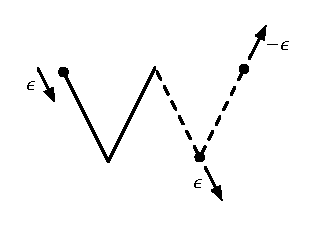
\includegraphics{images/dcjoin}
    \caption{\dcjoin}
    \figlabel{dcjoin}
  \end{figure}
  We have adapted the functional sub-term rule for positive subtyping and added the
  record sub-term rule. The functional sub-term rule \dcsubfun captures the invariance of argument types by
  equating the two argument types and propagates the co-variance of the return type.
  In the record sub-term rule \dcsubrec, the co-variance of the labels' types is propagated.
  We use a notational shortcut to differentiate between up and down distance. The up-distance regards
  the first type as a subtype of the second, whereas the down-distance regards the first type
  as a supertype of the second; thus if the
  up-distance between two records is observed ($\epsilon=+$), the record $\set{\vec{l}_-:\vec{\type{T}}_-}$
  ought to have more fields than $\set{\vec{l}_+:\vec{\type{T}}_+}$. We can therefore conclude by
  constraining all labels in $l_+=l_\epsilon$. The same reasoning applies for the other case.
  \begin{dfn}
    \dfnlabel{distanceconsistent}
    A constraint $C$ is said to be distance consistent whenever for each $\type{T}_1$,$\type{T}_2$
    in $\GTypes$ and for a natural number $n$ if $C\entailsdc d^\epsilon(\type{T}_1,\type{T}_2)\le n$ then
    $d_\GTypes^\epsilon(\type{T}_1,\type{T}_2)\le n$.
  \end{dfn}
  Distance consistency of a constraint $C$
  can be verified by constructing two $\mathcal{O}(\card{C})\times\mathcal{O}(\card{C})$
  arrays containing the up and down-distances between ground types. The inference system
  described before can then be used to find inconsistencies, if any, in $C$. The up
  and down-distances between ground types can be straightforwardly calculated, and we
  summarize the results here.
  \begin{mathpar}
    d^+(\type{T}, \top) =
      \left\{\begin{array}{cl} 0 & \type{T}=\top \\ 1 & \textrm{otherwise} \end{array}\right.\and
    d^+(\basetype_1,\basetype_2) =
      \left\{\begin{array}{cl} 0 & \basetype_1=\basetype_2 \\ 2 & \basetype_1\ne\basetype_2 \end{array}\right.\and
    d^+(\type{T}_1\fun\type{T}_2,\type{T}_1'\fun\type{T}_2') =
      \left\{\begin{array}{cl} d^+(\type{T}_2,\type{T}_2') & \type{T}_1=\type{T}_1' \\ 2 & \type{T}_1\ne\type{T}_1' \end{array}\right.\and
    d^+(\set{\vec{l}_1:\vec{\type{T}}_1},\set{\vec{l}_2:\vec{\type{T}}_2}) = \left\{\begin{array}{cl}
      0 & \set{\vec{l}_1:\vec{\type{T}}_1}=\set{\vec{l}_2:\vec{\type{T}}_2}\\
      1 & \bar{l}_2\subseteq\bar{l}_1\textrm{ and }\max_{l\in\bar{l}_2}{d^+(\type{T}_1^l,\type{T}_2^l)}\le 1\\
      2 & \textrm{otherwise} \end{array}\right.
  \end{mathpar}
  All other cases have an up-distance of $2$. The down-distance can be similarly calculated.
  \begin{mathpar}
    d^-(\top,\type{T}) =
      \left\{\begin{array}{cl} 0 & \type{T}=\top \\ 1 & \textrm{otherwise} \end{array}\right.\and
    d^-(\type{T},\top) =
      \left\{\begin{array}{cl} 0 & \type{T}=\top \\ 2 & \textrm{otherwise} \end{array}\right.\and
    d^-(\basetype_1,\basetype_2) =
      \left\{\begin{array}{cl} 0 & \basetype_1=\basetype_2 \\ 3 & \basetype_1\ne\basetype_2 \end{array}\right.\and
    d^-(\type{T}_1\fun\type{T}_2,\type{T}_1'\fun\type{T}_2') =
      \left\{\begin{array}{cl} d^-(\type{T}_2,\type{T}_2') & \type{T}_1=\type{T}_1' \\ 3 & \type{T}_1\ne\type{T}_1' \end{array}\right.\and
    d^-(\set{\vec{l}_1:\vec{\type{T}}_1},\set{\vec{l}_2:\vec{\type{T}}_2}) = \left\{\begin{array}{cl}
      0 & \set{\vec{l}_1:\vec{\type{T}}_1}=\set{\vec{l}_2:\vec{\type{T}}_2}\\
      1 & \bar{l}_1\subseteq\bar{l}_2\textrm{ and }\max_{l\in\bar{l}_1}{d^-(\type{T}_1^l,\type{T}_2^l)}\le 1\\
      3 & \bar{l}_1\cap\bar{l}_2\ne\emptyset\textrm{ and }\max_{l\in\bar{l}_1\cap\bar{l}_2}{d^-(\type{T}_1^l,\type{T}_2^l)}=3\\
      2 & \textrm{otherwise} \end{array}\right.
  \end{mathpar}
  All other cases have a down-distance of $3$.
  Benke \cite{benke93} showed that the two following theorems hold.
  \begin{thm}
    Distance consistency is NLOGSPACE complete.
  \end{thm}
  \begin{thm}
    A constraint is satisfiable if and only if it is weakly satisfiable and distance consistent.
  \end{thm}
  To highlight the separation of satisfiability into weak satisfiability and distance consistency
  we give two examples.
  The constraint $\Int\fun\type{X}\subtype\Int\fun\type{X}\fun\type{X}$ is distance consistent
  but not weakly satisfiable whereas the constraint $\Int\subtype\Bool$ is not distance consistent
  but weakly satisfiable.
  
  \chapter{Conclusion}
  \section{Related Work}
  Hindley/Milner type inference has been extended in numerous ways. For instance,
  Kfoury and Wells \cite{kfoury:rank2} consider inference for the rank-2 fragment
  of the second-order $\lambda$-calculus, later extended by Peyton Jones et al.
  \cite{peytonjones:rank} to arbitrary-rank types with the help of type annotations.
  
  Hofmann and Pierce \cite{pierce:positive-subtyping} introduce Positive Subtyping
  and enrich the traditional coercion interpretation of subtyping
  by adding an overwriting function. In addition to giving an equational theory
  for their calculus, they discuss differences between contra-variant subtyping
  and positive subtyping and give encodings of objects, interfaces and classes with
  self.
  
  Aiken and Wimmers \cite{aiken:ticti} consider type inclusion
  constraints and develop an algorithm to solve these constraints.
  In addition to the types we consider, they also include union types, intersection types,
  recursive types and a bottom type. However, they do not discuss complexity bounds.
  We believe that the algorithm they describe is applicable to the constraints
  that our type system produce, if the constraint simplification step were
  adapted to additionally constrain argument types to be positive.
  The type system we present is an instance of Sulzmann's HM(X) framework
  \cite{sulzmann97type}. In comparison, we present an effective algorithmic version
  of type inference and give complexity bounds.
  
  Palsberg \cite{palsberg94efficient} has shown that type inference
  for object types defined by Abadi and Cardelli \cite{abadi94theory}
  is PTIME-complete. In their object calculus, Abadi and Cardelli have width subtyping only
  and functional subtyping is invariant.
  Hoang and Mitchell \cite{hoang:lower-bounds} studied constraint satisfaction
  in presence of contra-variant subtyping and showed this problem can be PSPACE-hard.
  
  Pierce and Turner's \cite{PierceTurner:LTI,PierceTurner:LTI-FSUB} local type inference techniques,
  or their extension by Odersky et al. \cite{ozz:colored-local}, focus on the same
  problem as our system - type inference in presence of subtyping - with a very different approach.
  These techniques are local and thus require some type annotations from the programmer,
  but remove the burden of writing silly types. Embedding local inference in
  a programming language is simpler and more flexible than Hindley/Milner type
  inference and has been chosen for the programming language Scala \cite{scala}.
  A common pitfall of local techniques is the difficulty for
  a programmer to understand which type annotations are necessary.
  
  \section{Future Work}
  Switching back to our work, we now outline future directions.
  
  \noindent\textbf{Verifying Type Annotations}
  Allowing the programmer to give type annotations when interacting with
  the type system requires extra theory. These optional type annotations
  are given as type schemes, which must be typed
  in the polymorphic typing judgment. When type checking a program,
  the type system infers a type scheme, which ought to be checked against the
  type scheme provided by the programmer. Since our type system produces the most
  precise type (with respect to the subtyping relation on type schemes)
  for a term, we need to verify that the programmer's annotation
  is a supertype of the inferred type scheme. In our presentation, the subtyping relation
  on type schemes \dfnref{poly_subtype} is semantic and its implementation is thus not obvious.
  We would need to give an efficient algorithmic presentation of the semantic subtyping
  relation on type schemes.
  
  %It is the case that $\forall\bar{\type{X}}|C.\type{T}_1\subtype\forall\bar{\type{Y}}|D.\type{T}_2$ is equivalent to
  %$\exists\bar{\type{X}}\cup\bar{\type{Y}}.C\land D\land \type{T}_1\subtype\type{T}_2$ leading
  %us towards a simple satisfiability verification. The formalization is left as future work.
  
  
  \noindent\textbf{Recursive Types and Bottom Type}
  The constraint system we have presented is syntactic and we therefore fail
  to type all pure terms. The Y-combinator for instance
  $\lambda x.(\lambda y.y\ (x\ x))\ (\lambda y.y\ (x\ x))$ produces a constraint
  that is not satisfiable.
  
  Based on the work of Amadio and Cardelli \cite{amadiocardelli93},
  we would like to add recursive types to give a meaning to constraints
  of the form $\type{X}_1\fun\type{X}_2\subtype\type{X}_1$. It is nonetheless unclear
  how the efficiency of this extended system would compare to the one presented.
  
  A more direct extension is the addition of a minimal type bottom ($\bot$), dual to
  the maximal type top ($\top$). The efficiency of our system would be unchanged
  and similar challenges to the one discussed by Pierce \cite{Pierce:BQB} are
  present in our system with top, making the introduction of this additional
  type simple.
  
  \noindent\textbf{Simplifying Types}
  Constraint based type inference systems suffer from over-expressivity. Equivalent
  type schemes can take many shape and finding the ``best'' representation
  is non-trivial. In his work on bounded quantification with bottom, Pierce \cite{Pierce:BQB}
  alludes to similar difficulties in the syntactic representation of type schemes.
  
  The type system we present does produce type schemes that are difficult to read.
  Constraints are aggregated and verified for satisfiability but never simplified.
  In the appendix, we have included type derivations of typical expressions
  and the unusual size of the inferred type is eye-catching. We finish
  these type derivations by using the declarative rule \decsub, when needed,
  to highlight the possibilities for simplification. A type scheme $\forall\bar{\type{X}}'|C'.\type{T}'$
  is simpler than $\forall\bar{\type{X}}|C.\type{T}$ if it is equivalent
  but ``syntactically less verbose''. This definition is intentionally vague
  to give leeway for future work. We briefly discuss several
  ideas for simplifications, but leave as future work their
  formalization.
  
  \begin{itemize}
    \item Since we view constraints syntactically, and not as a set of subtyping
      inequalities, we must represent the empty constraint by $\true$. Whenever
      constraints are conjuncted (\sdrec, \sdsel, \sdapp) the $\true$ predicate
      could be eliminated instead of being carried forward.
    
    \item If a curried addition function is applied to a number, we would expect the
      type of the resulting expression to be $\Int\fun\Int$ but our type system infers
      $\type{S}=\forall\bar{\type{X}}|\Int\fun\Int\fun\Int\subtype\type{X}_1\fun\type{X}_2\land\Int\subtype\type{X}_1.\type{X}_2$
      whose useful solution is indeed $\Int\fun\Int$. Here, the original type schemes'
      interpretation $\sinterp{\type{S}}$ has a lower bound $\Int\fun\Int$
      which is as expressive as the type scheme itself. Whenever a lower bounded
      type scheme is inferred, the type inference system should use the lower bound
      instead of the more complex type scheme.
  
    \item Because of the way constraints are generated, extraneous type variables
      may be introduced. If the constraint $\type{X}_1\subtype\type{X}_2\land\type{X}_2\subtype\type{X}_3$
      appears in a type scheme whose monotype is $\type{X}_1\fun\type{X}_3$ then
      one could remove the intermediary $\type{X}_2$ type variable. Generally speaking,
      redundant constraints may be eliminated. Pottier and R\'emy \cite{pottier-remy-emlti}
      give standard constraint equivalence laws which can be easily complemented
      with subtyping specific equivalences.
  \end{itemize}
  
  Aside from these typical difficulties with constraint-based typings, positive
  subtyping adds challenges of its own. Aiken and Wimmers \cite{aiken:ticti}
  explain that in their type system, if a quantified type is monotonic
  (respectively anti-monotonic) in some type variable $\type{X}$, then
  $\type{X}$ can be instantiated to the lower bound (respectively upper bound)
  implied by the constraint without altering the meaning of the type scheme.
  This simplification is not meaning preserving with positive subtyping but
  instead could reduce the precision of a type scheme. The type of the
  apply function discussed in the introduction exhibits this behaviour:
  the inferred type scheme is
  \begin{displaymath}
    \forall\bar{\type{X}}|\type{X}_1\subtype\type{X}_2.\type{X}_1\fun(\type{X}_2\fun\type{X}_3)\fun\type{X}_3
  \end{displaymath}
  in which $\type{X}_1$ appears contra-variantly and $\type{X}_2$ appears co-variantly.
  We have seen previously that equating $\type{X}_1$ with $\type{X}_2$
  reduces the expressiveness of the overall type scheme. An interesting counter-point is the
  other version of the apply function taking the function first and then the value.
  Its inferred type is
  \begin{displaymath}
    \forall\bar{\type{X}}|\type{X}_3\subtype\type{X}_1.(\type{X}_1\fun\type{X}_2)\fun\type{X}_3\fun\type{X}_2
  \end{displaymath}
  which can be simplified to
  \begin{displaymath}
    \forall\bar{\type{X}}|\true.(\type{X}_1\fun\type{X}_2)\fun\type{X}_1\fun\type{X}_2
  \end{displaymath}
  since after the first application, the resulting type will be
  $\forall\emptyset|\true.\type{T}_1\fun\type{T}_2$ for some types $\type{T}_1$ and
  $\type{T}_2$. The subtyping flexibility provided by the removed constraint
  is provided by the application rule. We conjecture that Aiken and Wimmers' optimization applies
  to type variables whose upper bound appears first.
  
  To tackle this problem, we can regard curried functions' type as multi-instantiation types.
  Consider a curried function whose type is $\type{T}_1\fun\type{T}_2\fun\cdots\fun\type{T}_n$.
  When this function is first applied, the type system must decide
  the best choices for the type variables in $\type{T}_1$ (i.e. $\ftv(\type{T}_1)$).
  In another portion of the type derivation, the resulting expression may be applied again
  and the type system must now find the best choice for type variables in $\type{T}_2$,
  and so on. For preciseness, when instantiating $\type{T}_i$'s type variables,
  we must not restrict the range of $\type{T}_{i+1}\fun\cdots\fun\type{T}_n$.
  With positive subtyping, the types $\type{T}_1$ through $\type{T}_{n-1}$ are invariant,
  and the constraint is there to recover the lost flexibility. When simplifying the
  constraint, we need to be certain to preserve enough flexibility.
  
  \noindent\textbf{Post-inference Variance Analysis}
  Based on the observations about type simplification, it might be interesting
  to take a radically different approach. Instead of inferring a very general constrained type
  and simplifying it, we could infer a simple Hindley/Milner type
  and generalize it using a variance analysis.
  
  The Hindley/Milner type of the apply function $\lambda x.\lambda f.f\ x$ is
  $\forall\type{X},\type{Y}.\type{X}\fun(\type{X}\fun\type{Y})\fun\type{Y}$.
  With the standard subtyping relation, the first occurrence of the type
  variable $\type{X}$ is anti-monotonic whereas the second occurrence is
  monotonic. Since these two occurrences conflict and they appear at
  different instantiation times, one must introduce a constraint to increase
  the expressiveness of the resulting type scheme.
  
  Following this approach, one would have to fold subsumption
  into each typing rule to account for ground types. In the
  application rule for instance, if a function with type $\type{T}_1\fun\type{T}_2$
  is applied to a grounded type $\type{T}_1'$ we need to allow $\type{T}_1'$
  to be a subtype of $\type{T}_1$.
  
  In the early steps of this research, we considered a ``conformance'' based type
  system using a post-inference variance analysis when typing expressions.
  The conformance relation is an superset of the positive subtyping relation
  but a strict subset of the standard contra-variant relation. This approach
  benefits from type conciseness, but its other advantages are unclear.
  
  \noindent\textbf{Satisfiability of Constraints} Determining whether a constraint is
  satisfiable is key to the type inference's efficiency. We have show that constraint satisfiability
  is PTIME-complete and have presented a decomposition of this problem into weak satisfiability
  and distance consistency. We believe that a more direct algorithm tuned to the specific
  constraints generated by the type inference would be more effective in
  practice.
    
  \section{Conclusion}
  We have outlined the difficulties introduced by positive subtyping, a weaker
  notion of subtyping where contra-variant positions are forced to be
  invariant. We have proposed a constraint based type inference system to
  recover the lost expressiveness and showed that, in our setting,
  satisfiability of the constraints generated by the type inference
  is PTIME-complete.
  
  The programming language world is divided into two very separate communities,
  dynamically typed languages and statically typed languages. This divide
  goes back to Church and Curry, and has not weakened over the years.
  
  In statically typed languages, inference relieves the programmer
  from writing silly types. Hindley/Milner type inference has set the standard,
  but is difficult to extend and quickly becomes intractable or undecidable.
  In complex languages
  such as Scala \cite{scala} local inference, pioneered by Pierce and Turner
  \cite{PierceTurner:LTI}, is preferred. Until recently,
  mainstream programming languages did not benefit from these techniques.
  Despite the extensive background theory, introducing type inference and generics
  in Java \cite{bracha98making,java4} has been difficult and shown  buggy \cite{nominaltyping}.
  
  Statically typed languages are very well suited for large scale developments.
  The type system helps the programmer along the development cycle, allows
  for complex re-factoring and serves as a precise up-to-date documentation.
  In addition, statically typed languages can be aggressively optimized and
  thus very efficiently implemented.
  
  On the other hand, dynamically typed languages benefit from a fast-paced
  compilation-less programming cycle making software development
  simpler and at the reach of beginners. It also makes software development very
  lightweight, appropriate for software whose malleability is crucial.
  
  Making dynamically typed languages benefit from the research applicable to
  statically typed languages is a challenge of its own. Flanagan \cite{hybrid}
  introduced the concept of hybrid typing, later extended to gradual typing
  by Siek and Taha \cite{gradual}. Rather than aiming at total type inference - undecidable
  for languages in which method override, removal and update is permitted -
  gradual typing partially infers types and leaves unknown types to
  be dynamically checked. This approach gives soft guarantees to programmers
  who can benefit from a fast paced prototyping phase and later add a few
  type annotations to crystallize their thinking, easing re-factoring and
  extendibility.
  
  In this evolution, we see positive subtyping as one approach to tackle
  the complex structural subtyping relations induced by dynamically typed
  languages and thus improve the scope and preciseness of type inference
  in languages built for other purposes.
  
  \appendix
  \chapter{Typing Examples}
  We give a few examples from our prototype implementation\footnote{
    The implementation is a work in progress and the distance consistency check
    is not yet incorporated.}
  accessible on \url{http://www.stanford.edu/~plperez/}.
  The syntax used is close to the programming language ML. Constants comprises
  integers (e.g. \verb+14+), booleans (\verb+true+ or \verb+false+) and characters
  (e.g. \verb+`a'+). Our system infers type schemes which are typed
  in the polymorphic typing judgment.
  Our first example is the identity function:
  \begin{verbatim}fn x => x : \X1|true.X1 -> X1\end{verbatim}
  The inferred type is the usual Hindley/Milner type. Our system
  prints type schemes as \verb+\X|C.T+ where \verb+X+ is the set of quantified
  type variables, \verb+C+ is the constraint and \verb+T+ is the monomorphic
  type. We simplify slightly the constraint for presentation.
  We now show an example of record selection, where the record type
  is extracted instead of adding a constraint.
  \begin{verbatim}#l {l=3} : \0|true.Int\end{verbatim}
  In comparison, the selection function constrains the type variable
  representing the argument type.
  \begin{verbatim}fn x => #l x : \X1,X2|X1 <: {l:X2}.X1 -> X2\end{verbatim}
  Our next example is the the Church encoding of a boolean
  $\lambda x.\lambda y.x$.
  \begin{verbatim}fn x => fn y => x : \X1,X2|true.X1 -> X2 -> X1\end{verbatim}
  Its inferred type  is similar to the Hindley/Milner type.
  In comparison with Aiken and Wimmers \cite{aiken:ticti}, the type variable
  \verb+X2+ cannot be instantiated to top as it appears in an invariant position.
  The apply function ($\lambda x.\lambda f.f\ x$) taking a value and then a function
  has the type discussed earlier, but the presentation is not as terse.
  \begin{verbatim}fn x => fn f => f x : \X1,X2,X3,X4|X1 <: X3 ^ X2 <: X3 -> X4.X1 -> X2 -> X4\end{verbatim}
  To highlight let-polymorphism, we can apply the identity function to
  constants with different types.
  %\carriagereturn
  \begin{verbatim}let id = fn x => x in (fn w => id `a') (id true) end :
    \X1,X2,X3|Bool <: X3 ^ X3 <: X1 ^ Char <: X2.X2\end{verbatim}
  We use $(\lambda w.e_2)\ e_1$ as the consecution operator.
  Each individual constraint corresponds to one application and could
  be simplified when presenting the type scheme.
  
  \chapter{Type Derivations Examples}
  \section{Identity Function}
  \begin{mathpar}
    \inferrule{
      \inferrule*[Left=$\Delta_1$]{
        \inferrule{
          \inferrule{
            \lrp{x:\forall\emptyset|\true.\type{X}}(x)=\forall\emptyset|\true.\type{X}
          }{x:\forall\emptyset|\true.\type{X}\entailsp x:\forall\emptyset|\true.\type{X}}
        }{\true;x:\forall\emptyset|\true.\type{X}\entailsm x:\type{X}}
      }{\true;\emptyset\entailsm\lambda x.x:\type{X}\fun\type{X}}
    }{\emptyset\entailsp\lambda x.x:\forall\type{X}|\true.\type{X}\fun\type{X}}
  \end{mathpar}
  
  \section{Identity Function applied to a Record}
  \begin{mathpar}
    \inferrule{
      \inferrule{
        \inferrule{
          \inferrule{
            \Delta_1
          }{\true;\emptyset\entailsm\lambda x.x:\type{X}\fun\type{X}}\and
          \inferrule{
            \inferrule{
              \inferrule{
                \Base(4)=\Int
              }{\emptyset\entailsp 4:\forall\emptyset|\true.\Int}
            }{\true;\emptyset\entailsm 4:\Int}
          }{\true;\emptyset\entailsm\set{l=4}:\set{l:\Int}}
        }{\true\land\true\land\type{X}\fun\type{X}\subtype\type{Y}_1\fun\type{Y}_2\land\set{l:\Int}\subtype\type{Y}_1;\emptyset\entailsm\lambda x.x\ \set{l=4}:\type{Y}_2}
      }{\emptyset\entailsp\lambda x.x\ \set{l=4}:\forall\set{\type{X},\type{Y}_1,\type{Y}_2}|\true\land\true\land\type{X}\fun\type{X}\subtype\type{Y}_1\fun\type{Y}_2\land\set{l:\Int}\subtype\type{Y}_1.\type{Y}_2}
    }{\emptyset\entailsp\lambda x.x\ \set{l=4}:\forall\emptyset|\true.\set{l:\Int}}
  \end{mathpar}
  
  \section{Increment Function}
  \begin{mathpar}
    \inferrule{
      \inferrule{
        \inferrule{
          \inferrule{
            \inferrule{
              \inferrule{
                \vdots
              }{\entailsm +:\Int\fun\Int\fun\Int}\and
              \inferrule{
                \vdots
              }{\entailsm x:\type{X}_1}
            }{\ensuremath{\overbrace{\Int\fun\Int\fun\Int\subtype\type{X}_2\fun\type{X}_3\land\type{X}_1\subtype\type{X}_2}^{C_1}};x:\forall\emptyset|\true.\type{X}_1\entailsm x+:\type{X}_3}\and
            \inferrule{
              \vdots
            }{\entailsm 1:\Int}
          }{\ensuremath{\overbrace{C_1\land\type{X}_3\subtype\type{X}_4\fun\type{X}_5\land\type{X}_3\subtype\type{X}_4}^{C_2}};x:\forall\emptyset|\true.\type{X}_1\entailsm x+1:\type{X}_5}
        }{C_2;\emptyset\entailsm\lambda x.x+1:\type{X}_1\fun\type{X}_5}
      }{\emptyset\entailsp\lambda x.x+1:\forall\bar{\type{X}}|C_2.\type{X}_1\fun\type{X}_5}
    }{\emptyset\entailsp\lambda x.x+1:\forall\emptyset|\true.\Int\fun\Int}
  \end{mathpar}
  
  \section{Selection Function}
  \begin{mathpar}
    \inferrule{
      \inferrule{
        \inferrule{
          \inferrule{
            \inferrule{
              \vdots
            }{\true;x:\forall\emptyset|\true.\type{X}_1\entailsm x:\type{X}_1}
          }{\true\land\type{X}_1\subtype\set{l:\type{X}_2};x:\forall\emptyset|\true.\type{X}_1\entailsm x.l:\type{X}_2}
        }{\true\land\type{X}_1\subtype\set{l:\type{X}_2};\emptyset\entailsm\lambda x.x.l:\type{X}_1\fun\type{X}_2}
      }{\emptyset\entailsp\lambda x.x.l:\forall\bar{\type{X}}|\true\land\type{X}_1\subtype\set{l:\type{X}_2}.\type{X}_1\fun\type{X}_2}
    }{\emptyset\entailsp\lambda x.x.l:\forall\type{X}|\true.\set{l:\type{X}}\fun\type{X}}
  \end{mathpar}
  
  \section{Apply Function ($f$ then $d$)}
  \begin{mathpar}
    \inferrule{
      \inferrule{
        \inferrule{
          \inferrule{
            \inferrule{
              \inferrule{
                \vdots
              }{\true;\Gamma\entailsm f:\type{X}_1}\and
              \inferrule{
                \vdots
              }{\true;\Gamma\entailsm d:\type{X}_2}
            }{\ensuremath{\overbrace{\type{X}_1\subtype\type{X}_3\fun\type{X}_4\land\type{X}_2\subtype\type{X}_3}^{C}};\ensuremath{\overbrace{f:\forall\emptyset|\true.\type{X}_1\cdot d:\forall\emptyset|\true.\type{X}_2}^\Gamma}\entailsm f\ d:\type{X}_4}
          }{C;f:\forall\emptyset|\true.\type{X}_1\entailsm\lambda d.f\ d:\type{X}_2\fun\type{X}_4}
        }{C;\emptyset\entailsm\lambda f.\lambda d.f\ d:\type{X}_1\fun\type{X}_2\fun\type{X}_4}
      }{\emptyset\entailsp\lambda f.\lambda d.f\ d:\forall\bar{\type{X}}|C.\type{X}_1\fun\type{X}_2\fun\type{X}_4}
    }{\emptyset\entailsp\lambda f.\lambda d.f\ d:\forall\bar{\type{X}}|\true.(\type{X}_1\fun\type{X}_2)\fun\type{X}_1\fun\type{X}_2}
  \end{mathpar}
  
  \section{Apply Function ($d$ then $f$)}
  \begin{mathpar}
    \inferrule{
      \inferrule{
        \inferrule{
          \inferrule{
            \inferrule{
              \inferrule{
                \vdots
              }{\true;\Gamma\entailsm f:\type{X}_2}\and
              \inferrule{
                \vdots
              }{\true;\Gamma\entailsm d:\type{X}_1}
            }{\ensuremath{\overbrace{\type{X}_2\subtype\type{X}_3\fun\type{X}_4\land\type{X}_1\subtype\type{X}_3}^{C}};\ensuremath{\overbrace{d:\forall\emptyset|\true.\type{X}_1\cdot f:\forall\emptyset|\true.\type{X}_2}^\Gamma}\entailsm f\ d:\type{X}_4}
          }{C;d:\forall\emptyset|\true.\type{X}_1\entailsm\lambda f.f\ d:\type{X}_1\fun\type{X}_4}
        }{C;\emptyset\entailsm\lambda d.\lambda f.f\ d:\type{X}_2\fun\type{X}_1\fun\type{X}_4}
      }{\emptyset\entailsp\lambda d.\lambda f.f\ d:\forall\bar{\type{X}}|C.\type{X}_2\fun\type{X}_1\fun\type{X}_4}
    }{\emptyset\entailsp\lambda d.\lambda f.f\ d:\forall\bar{\type{X}}|\type{X}_1\subtype\type{X}_2.\type{X}_1\fun(\type{X}_2\fun\type{X}_3)\fun\type{X}_3}
  \end{mathpar}
  
  \chapter{Notations}
  \listofnotations{notations}
  
  \nocite{*}
  \bibliographystyle{plain}
  \bibliography{work}
\end{document}
